\pdfoutput=1
%% Author: PGL  Porta Mana, ALS Filipowicz
%% Created: 2018-04-08T16:54:19+0200
%% Last-Updated: 2018-05-29T22:35:07+0200
%%%%%%%%%%%%%%%%%%%%%%%%%%%%%%%%%%%%%%%%%%%%%%%%%%%%%%%%%%%%%%%%%%%%%%
% Report-no: ***
\newif\ifarxiv
\arxivfalse
\ifarxiv\pdfmapfile{+classico.map}\fi
\newif\ifafour
\afourfalse % true = A4, false = A5
\newif\iftypodisclaim % typographical disclaim on the side
\typodisclaimtrue
\newif\ifpublic
\publicfalse % true = for publication, false = personal notes
\newcommand*{\memfontfamily}{zplx}
\newcommand*{\memfontpack}{newpxtext}
\documentclass[\ifafour a4paper,12pt,\else a5paper,10pt,\fi%extrafontsizes,%
onecolumn,oneside,article,%french,italian,german,swedish,latin,
british%
]{memoir}
\newcommand*{\oggi}{\today}
\newcommand*{\firstdraft}{14 April 2018}
\newcommand*{\firstpublished}{\oggi}
\newcommand*{\propertitle}{Bayesian Plinko\\{\large Study notes}}
\newcommand*{\pdftitle}{Bayesian Plinko}
\newcommand*{\headtitle}{Bayesian Plinko}
\newcommand*{\pdfauthor}{A. L. S. Filipowicz, P.G.L.  Porta Mana, Y. Roudi,
  et al.}
\newcommand*{\etal}{{et al.}}
\newcommand*{\headauthor}{\ifpublic Filipowicz \amp\ Porta Mana%
\else Alex \etal\fi}
\newcommand*{\reporthead}{}
%%%%%%%%%%%%%%%%%%%%%%%%%%%%%%%%%%%%%%%%%%%%%%%%%%%%%%%%%%%%%%%%%%%%%%%%%%%%
%%%%%%%%%%%%%%%%%%%%%%%%%%%%%%%%%%%%%%%%%%%%%%%%%%%%%%%%%%%%%%%%%%%%%%%%%%%%
%\usepackage{pifont}
%\usepackage{fontawesome}
\usepackage[T1]{fontenc} 
\input{glyphtounicode} \pdfgentounicode=1
\usepackage[utf8]{inputenx}
%\usepackage{newunicodechar}
% \newunicodechar{Ĕ}{\u{E}}
% \newunicodechar{ĕ}{\u{e}}
% \newunicodechar{Ĭ}{\u{I}}
% \newunicodechar{ĭ}{\u{\i}}
% \newunicodechar{Ŏ}{\u{O}}
% \newunicodechar{ŏ}{\u{o}}
% \newunicodechar{Ŭ}{\u{U}}
% \newunicodechar{ŭ}{\u{u}}
% \newunicodechar{Ā}{\=A}
% \newunicodechar{ā}{\=a}
% \newunicodechar{Ē}{\=E}
% \newunicodechar{ē}{\=e}
% \newunicodechar{Ī}{\=I}
% \newunicodechar{ī}{\={\i}}
% \newunicodechar{Ō}{\=O}
% \newunicodechar{ō}{\=o}
% \newunicodechar{Ū}{\=U}
% \newunicodechar{ū}{\=u}
% \newunicodechar{Ȳ}{\=Y}
% \newunicodechar{ȳ}{\=y}

\newcommand*{\bmmax}{0} % reduce number of bold fonts, before bm
\newcommand*{\hmmax}{0} % reduce number of heavy fonts, before bm
\usepackage{textcomp}
\usepackage[normalem]{ulem}
% \makeatletter
% \def\ssout{\bgroup \ULdepth=-.35ex%\UL@setULdepth
%  \markoverwith{\lower\ULdepth\hbox
%    {\kern-.03em\vbox{\hrule width.2em\kern1.2\p@\hrule}\kern-.03em}}%
%  \ULon}
% \makeatother
\usepackage{amsmath}
\usepackage{mathtools}
\usepackage{empheq}% automatically calls amsmath and mathtools
\newcommand*{\widefbox}[1]{\fbox{\hspace{1em}#1\hspace{1em}}}
\setlength{\multlinegap}{0pt}
%\usepackage{fancybox}
\usepackage{framed}
% \usepackage[misc]{ifsym} % for dice
% \newcommand*{\diceone}{{\scriptsize\Cube{1}}}
\usepackage{amssymb}
\usepackage{amsxtra}

\usepackage[main=british,french,italian,german,swedish,latin,esperanto]{babel}\selectlanguage{british}
\newcommand*{\langfrench}{\foreignlanguage{french}}
\newcommand*{\langgerman}{\foreignlanguage{german}}
\newcommand*{\langitalian}{\foreignlanguage{italian}}
\newcommand*{\langswedish}{\foreignlanguage{swedish}}
\newcommand*{\langlatin}{\foreignlanguage{latin}}
\newcommand*{\langnohyph}{\foreignlanguage{nohyphenation}}

\usepackage[autostyle=false,autopunct=false,english=british]{csquotes}
\setquotestyle{british}

\usepackage{amsthm}
\newcommand*{\QED}{\textsc{q.e.d.}}
\renewcommand*{\qedsymbol}{\QED}
\theoremstyle{remark}
\newtheorem{note}{Note}
\newtheorem*{remark}{Note}
\newtheoremstyle{innote}{\parsep}{\parsep}{\footnotesize}{}{}{}{0pt}{}
\theoremstyle{innote}
\newtheorem*{innote}{}


\usepackage[shortlabels,inline]{enumitem}
\SetEnumitemKey{para}{itemindent=\parindent,leftmargin=0pt,listparindent=\parindent,parsep=0pt,itemsep=\topsep}
% \begin{asparaenum} = \begin{enumerate}[para]
% \begin{inparaenum} = \begin{enumerate*}
\setlist[enumerate,2]{label=\alph*.}
\setlist[enumerate]{leftmargin=\parindent}
\setlist[itemize]{leftmargin=\parindent}
\setlist[description]{leftmargin=\parindent}

\usepackage[babel,theoremfont]{newpxtext}
\usepackage[bigdelims,nosymbolsc%,smallerops % probably arXiv doesn't have it
]{newpxmath}
\useosf\linespread{1.083}
%% smaller operators for old version of newpxmath
\makeatletter
\def\re@DeclareMathSymbol#1#2#3#4{%
    \let#1=\undefined
    \DeclareMathSymbol{#1}{#2}{#3}{#4}}
%\re@DeclareMathSymbol{\bigsqcupop}{\mathop}{largesymbols}{"46}
%\re@DeclareMathSymbol{\bigodotop}{\mathop}{largesymbols}{"4A}
\re@DeclareMathSymbol{\bigoplusop}{\mathop}{largesymbols}{"4C}
\re@DeclareMathSymbol{\bigotimesop}{\mathop}{largesymbols}{"4E}
\re@DeclareMathSymbol{\sumop}{\mathop}{largesymbols}{"50}
\re@DeclareMathSymbol{\prodop}{\mathop}{largesymbols}{"51}
\re@DeclareMathSymbol{\bigcupop}{\mathop}{largesymbols}{"53}
\re@DeclareMathSymbol{\bigcapop}{\mathop}{largesymbols}{"54}
%\re@DeclareMathSymbol{\biguplusop}{\mathop}{largesymbols}{"55}
\re@DeclareMathSymbol{\bigwedgeop}{\mathop}{largesymbols}{"56}
\re@DeclareMathSymbol{\bigveeop}{\mathop}{largesymbols}{"57}
%\re@DeclareMathSymbol{\bigcupdotop}{\mathop}{largesymbols}{"DF}
%\re@DeclareMathSymbol{\bigcapplusop}{\mathop}{largesymbolsPXA}{"00}
%\re@DeclareMathSymbol{\bigsqcupplusop}{\mathop}{largesymbolsPXA}{"02}
%\re@DeclareMathSymbol{\bigsqcapplusop}{\mathop}{largesymbolsPXA}{"04}
%\re@DeclareMathSymbol{\bigsqcapop}{\mathop}{largesymbolsPXA}{"06}
\re@DeclareMathSymbol{\bigtimesop}{\mathop}{largesymbolsPXA}{"10}
%\re@DeclareMathSymbol{\coprodop}{\mathop}{largesymbols}{"60}
%\re@DeclareMathSymbol{\varprod}{\mathop}{largesymbolsPXA}{16}
\makeatother


%% With euler font cursive for Greek letters - the [1] means 100% scaling
\DeclareFontFamily{U}{egreek}{\skewchar\font'177}%
\DeclareFontShape{U}{egreek}{m}{n}{<-6>s*[1]eurm5 <6-8>s*[1]eurm7 <8->s*[1]eurm10}{}%
\DeclareFontShape{U}{egreek}{m}{it}{<->s*[1]eurmo10}{}%
\DeclareFontShape{U}{egreek}{b}{n}{<-6>s*[1]eurb5 <6-8>s*[1]eurb7 <8->s*[1]eurb10}{}%
\DeclareFontShape{U}{egreek}{b}{it}{<->s*[1]eurbo10}{}%
\DeclareSymbolFont{egreeki}{U}{egreek}{m}{it}%
\SetSymbolFont{egreeki}{bold}{U}{egreek}{b}{it}% from the amsfonts package
\DeclareSymbolFont{egreekr}{U}{egreek}{m}{n}%
\SetSymbolFont{egreekr}{bold}{U}{egreek}{b}{n}% from the amsfonts package
% Take also \sum, \prod, \coprod symbols from Euler fonts
\DeclareFontFamily{U}{egreekx}{\skewchar\font'177}
\DeclareFontShape{U}{egreekx}{m}{n}{%
       <-7.5>s*[0.9]euex7%
    <7.5-8.5>s*[0.9]euex8%
    <8.5-9.5>s*[0.9]euex9%
    <9.5->s*[0.9]euex10%
}{}
\DeclareSymbolFont{egreekx}{U}{egreekx}{m}{n}
\DeclareMathSymbol{\sumop}{\mathop}{egreekx}{"50}
\DeclareMathSymbol{\prodop}{\mathop}{egreekx}{"51}
\DeclareMathSymbol{\coprodop}{\mathop}{egreekx}{"60}
\makeatletter
\def\sum{\DOTSI\sumop\slimits@}
\def\prod{\DOTSI\prodop\slimits@}
\def\coprod{\DOTSI\coprodop\slimits@}
\makeatother
\ifarxiv\else\let\varpartial\undefined
\let\partialup\undefined
\let\alpha\undefined
\let\beta\undefined
\let\gamma\undefined
\let\delta\undefined
\let\epsilon\undefined
\let\zeta\undefined
\let\eta\undefined
\let\theta\undefined
\let\iota\undefined
\let\kappa\undefined
\let\lambda\undefined
\let\mu\undefined
\let\nu\undefined
\let\xi\undefined
\let\omicron\undefined
\let\pi\undefined
\let\rho\undefined
\let\sigma\undefined
\let\tau\undefined
\let\upsilon\undefined
\let\phi\undefined
\let\chi\undefined
\let\psi\undefined
\let\omega\undefined
\let\varepsilon\undefined
\let\vartheta\undefined
\let\varpi\undefined
\let\varrho\undefined 
\let\varsigma\undefined
\let\varkappa\undefined
\let\varphi\undefined
%
\let\varAlpha\undefined
\let\varBeta\undefined
\let\varGamma\undefined
\let\varDelta\undefined
\let\varEpsilon\undefined
\let\varZeta\undefined
\let\varEta\undefined
\let\varTheta\undefined
\let\varIota\undefined
\let\varKappa\undefined
\let\varLambda\undefined
\let\varMu\undefined
\let\varNu\undefined
\let\varXi\undefined
\let\varOmicron\undefined
\let\varPi\undefined
\let\varRho\undefined
\let\varSigma\undefined
\let\varTau\undefined
\let\varUpsilon\undefined
\let\varPhi\undefined
\let\varChi\undefined
\let\varPsi\undefined
\let\varOmega\undefined
%
\let\Alpha\undefined
\let\Beta\undefined
\let\Gamma\undefined
\let\Delta\undefined
\let\Epsilon\undefined
\let\Zeta\undefined
\let\Eta\undefined
\let\Theta\undefined
\let\Iota\undefined
\let\Kappa\undefined
\let\Lambda\undefined
\let\Mu\undefined
\let\Nu\undefined
\let\Xi\undefined
\let\Omicron\undefined
\let\Pi\undefined
\let\Rho\undefined
\let\Sigma\undefined
\let\Tau\undefined
\let\Upsilon\undefined
\let\Phi\undefined
\let\Chi\undefined
\let\Psi\undefined
\let\Omega\undefined
%
\let\alphaup\undefined
\let\betaup\undefined
\let\gammaup\undefined
\let\deltaup\undefined
\let\epsilonup\undefined
\let\zetaup\undefined
\let\etaup\undefined
\let\thetaup\undefined
\let\iotaup\undefined
\let\kappaup\undefined
\let\lambdaup\undefined
\let\muup\undefined
\let\nuup\undefined
\let\xiup\undefined
\let\omicronup\undefined
\let\piup\undefined
\let\rhoup\undefined
\let\sigmaup\undefined
\let\tauup\undefined
\let\upsilonup\undefined
\let\phiup\undefined
\let\chiup\undefined
\let\psiup\undefined
\let\omegaup\undefined
\let\varepsilonup\undefined
\let\varthetaup\undefined
\let\varpiup\undefined
\let\varrhoup\undefined
\let\varsigmaup\undefined
\let\varkappaup\undefined
\let\varphiup\undefined
\fi% make sure no CMF greek letters sneak in
% Greek letters not usually given in LaTeX. Comment the unneeded ones
% \DeclareMathSymbol{\varpartial}{\mathalpha}{egreeki}{"40}
 \DeclareMathSymbol{\partialup}{\mathalpha}{egreekr}{"40}
% \DeclareMathSymbol{\alpha}{\mathalpha}{egreeki}{"0B}
% \DeclareMathSymbol{\beta}{\mathalpha}{egreeki}{"0C}
% \DeclareMathSymbol{\gamma}{\mathalpha}{egreeki}{"0D}
% \DeclareMathSymbol{\delta}{\mathalpha}{egreeki}{"0E}
 \DeclareMathSymbol{\epsilon}{\mathalpha}{egreeki}{"0F}
% \DeclareMathSymbol{\zeta}{\mathalpha}{egreeki}{"10}
% \DeclareMathSymbol{\eta}{\mathalpha}{egreeki}{"11}
 \DeclareMathSymbol{\theta}{\mathalpha}{egreeki}{"12}
% \DeclareMathSymbol{\iota}{\mathalpha}{egreeki}{"13}
 \DeclareMathSymbol{\kappa}{\mathalpha}{egreeki}{"14}
 \DeclareMathSymbol{\lambda}{\mathalpha}{egreeki}{"15}
 \DeclareMathSymbol{\mu}{\mathalpha}{egreeki}{"16}
 \DeclareMathSymbol{\nu}{\mathalpha}{egreeki}{"17}
% \DeclareMathSymbol{\xi}{\mathalpha}{egreeki}{"18}
% \DeclareMathSymbol{\omicron}{\mathalpha}{egreeki}{"6F}
% \DeclareMathSymbol{\pi}{\mathalpha}{egreeki}{"19}
% \DeclareMathSymbol{\rho}{\mathalpha}{egreeki}{"1A}
% \DeclareMathSymbol{\sigma}{\mathalpha}{egreeki}{"1B}
% \DeclareMathSymbol{\tau}{\mathalpha}{egreeki}{"1C}
% \DeclareMathSymbol{\upsilon}{\mathalpha}{egreeki}{"1D}
% \DeclareMathSymbol{\phi}{\mathalpha}{egreeki}{"1E}
 \DeclareMathSymbol{\chi}{\mathalpha}{egreeki}{"1F}
% \DeclareMathSymbol{\psi}{\mathalpha}{egreeki}{"20}
% \DeclareMathSymbol{\omega}{\mathalpha}{egreeki}{"21}
% \DeclareMathSymbol{\varepsilon}{\mathalpha}{egreeki}{"22}
% \DeclareMathSymbol{\vartheta}{\mathalpha}{egreeki}{"23}
% \DeclareMathSymbol{\varpi}{\mathalpha}{egreeki}{"24}
% \let\varrho\rho 
% \let\varsigma\sigma
 \let\varkappa\kappa
% \DeclareMathSymbol{\varphi}{\mathalpha}{egreeki}{"27}
% %
% \DeclareMathSymbol{\varAlpha}{\mathalpha}{egreeki}{"41}
% \DeclareMathSymbol{\varBeta}{\mathalpha}{egreeki}{"42}
% \DeclareMathSymbol{\varGamma}{\mathalpha}{egreeki}{"00}
 \DeclareMathSymbol{\varDelta}{\mathalpha}{egreeki}{"01}
 \DeclareMathSymbol{\varEpsilon}{\mathalpha}{egreeki}{"45}
% \DeclareMathSymbol{\varZeta}{\mathalpha}{egreeki}{"5A}
% \DeclareMathSymbol{\varEta}{\mathalpha}{egreeki}{"48}
 \DeclareMathSymbol{\varTheta}{\mathalpha}{egreeki}{"02}
 \DeclareMathSymbol{\varIota}{\mathalpha}{egreeki}{"49}
% \DeclareMathSymbol{\varKappa}{\mathalpha}{egreeki}{"4B}
 \DeclareMathSymbol{\varLambda}{\mathalpha}{egreeki}{"03}
% \DeclareMathSymbol{\varMu}{\mathalpha}{egreeki}{"4D}
% \DeclareMathSymbol{\varNu}{\mathalpha}{egreeki}{"4E}
% \DeclareMathSymbol{\varXi}{\mathalpha}{egreeki}{"04}
% \DeclareMathSymbol{\varOmicron}{\mathalpha}{egreeki}{"4F}
% \DeclareMathSymbol{\varPi}{\mathalpha}{egreeki}{"05}
% \DeclareMathSymbol{\varRho}{\mathalpha}{egreeki}{"50}
% \DeclareMathSymbol{\varSigma}{\mathalpha}{egreeki}{"06}
% \DeclareMathSymbol{\varTau}{\mathalpha}{egreeki}{"54}
% \DeclareMathSymbol{\varUpsilon}{\mathalpha}{egreeki}{"07}
% \DeclareMathSymbol{\varPhi}{\mathalpha}{egreeki}{"08}
% \DeclareMathSymbol{\varChi}{\mathalpha}{egreeki}{"58}
% \DeclareMathSymbol{\varPsi}{\mathalpha}{egreeki}{"09}
% \DeclareMathSymbol{\varOmega}{\mathalpha}{egreeki}{"0A} 
% %
% \DeclareMathSymbol{\Alpha}{\mathalpha}{egreekr}{"41}
% \DeclareMathSymbol{\Beta}{\mathalpha}{egreekr}{"42}
 \DeclareMathSymbol{\Gamma}{\mathalpha}{egreekr}{"00}
% \DeclareMathSymbol{\Delta}{\mathalpha}{egreekr}{"01}
% \DeclareMathSymbol{\Epsilon}{\mathalpha}{egreekr}{"45}
% \DeclareMathSymbol{\Zeta}{\mathalpha}{egreekr}{"5A}
% \DeclareMathSymbol{\Eta}{\mathalpha}{egreekr}{"48}
% \DeclareMathSymbol{\Theta}{\mathalpha}{egreekr}{"02}
% \DeclareMathSymbol{\Iota}{\mathalpha}{egreekr}{"49}
% \DeclareMathSymbol{\Kappa}{\mathalpha}{egreekr}{"4B}
% \DeclareMathSymbol{\Lambda}{\mathalpha}{egreekr}{"03}
% \DeclareMathSymbol{\Mu}{\mathalpha}{egreekr}{"4D}
% \DeclareMathSymbol{\Nu}{\mathalpha}{egreekr}{"4E}
% \DeclareMathSymbol{\Xi}{\mathalpha}{egreekr}{"04}
% \DeclareMathSymbol{\Omicron}{\mathalpha}{egreekr}{"4F}
% \DeclareMathSymbol{\Pi}{\mathalpha}{egreekr}{"05}
% \DeclareMathSymbol{\Rho}{\mathalpha}{egreekr}{"50}
% \DeclareMathSymbol{\Sigma}{\mathalpha}{egreekr}{"06}
% \DeclareMathSymbol{\Tau}{\mathalpha}{egreekr}{"54}
% \DeclareMathSymbol{\Upsilon}{\mathalpha}{egreekr}{"07}
% \DeclareMathSymbol{\Phi}{\mathalpha}{egreekr}{"08}
% \DeclareMathSymbol{\Chi}{\mathalpha}{egreekr}{"58}
% \DeclareMathSymbol{\Psi}{\mathalpha}{egreekr}{"09}
% \DeclareMathSymbol{\Omega}{\mathalpha}{egreekr}{"0A}
% %
% \DeclareMathSymbol{\alphaup}{\mathalpha}{egreekr}{"0B}
% \DeclareMathSymbol{\betaup}{\mathalpha}{egreekr}{"0C}
% \DeclareMathSymbol{\gammaup}{\mathalpha}{egreekr}{"0D}
 \DeclareMathSymbol{\deltaup}{\mathalpha}{egreekr}{"0E}
% \DeclareMathSymbol{\epsilonup}{\mathalpha}{egreekr}{"0F}
% \DeclareMathSymbol{\zetaup}{\mathalpha}{egreekr}{"10}
% \DeclareMathSymbol{\etaup}{\mathalpha}{egreekr}{"11}
% \DeclareMathSymbol{\thetaup}{\mathalpha}{egreekr}{"12}
% \DeclareMathSymbol{\iotaup}{\mathalpha}{egreekr}{"13}
% \DeclareMathSymbol{\kappaup}{\mathalpha}{egreekr}{"14}
% \DeclareMathSymbol{\lambdaup}{\mathalpha}{egreekr}{"15}
% \DeclareMathSymbol{\muup}{\mathalpha}{egreekr}{"16}
% \DeclareMathSymbol{\nuup}{\mathalpha}{egreekr}{"17}
% \DeclareMathSymbol{\xiup}{\mathalpha}{egreekr}{"18}
% \DeclareMathSymbol{\omicronup}{\mathalpha}{egreekr}{"6F}
  \DeclareMathSymbol{\piup}{\mathalpha}{egreekr}{"19}
% \DeclareMathSymbol{\rhoup}{\mathalpha}{egreekr}{"1A}
% \DeclareMathSymbol{\sigmaup}{\mathalpha}{egreekr}{"1B}
% \DeclareMathSymbol{\tauup}{\mathalpha}{egreekr}{"1C}
% \DeclareMathSymbol{\upsilonup}{\mathalpha}{egreekr}{"1D}
% \DeclareMathSymbol{\phiup}{\mathalpha}{egreekr}{"1E}
% \DeclareMathSymbol{\chiup}{\mathalpha}{egreekr}{"1F}
% \DeclareMathSymbol{\psiup}{\mathalpha}{egreekr}{"20}
% \DeclareMathSymbol{\omegaup}{\mathalpha}{egreekr}{"21}
% \DeclareMathSymbol{\varepsilonup}{\mathalpha}{egreekr}{"22}
% \DeclareMathSymbol{\varthetaup}{\mathalpha}{egreekr}{"23}
% \DeclareMathSymbol{\varpiup}{\mathalpha}{egreekr}{"24}
% \let\varrhoup\rhoup 
% \let\varsigmaup\sigmaup
% \let\varkappaup\kappaup
% \DeclareMathSymbol{\varphiup}{\mathalpha}{egreekr}{"27}

% Optima as sans-serif font
%\usepackage%[scaled=0.9]%
%{classico}
\renewcommand\sfdefault{uop}
\DeclareMathAlphabet{\mathsf}  {T1}{\sfdefault}{m}{sl}
\SetMathAlphabet{\mathsf}{bold}{T1}{\sfdefault}{b}{sl}
\newcommand*{\mathte}[1]{\textbf{\textit{\textsf{#1}}}}
% Upright sans-serif math alphabet
% \DeclareMathAlphabet{\mathsu}  {T1}{\sfdefault}{m}{n}
% \SetMathAlphabet{\mathsu}{bold}{T1}{\sfdefault}{b}{n}

% DejaVu Mono as typewriter text
\usepackage[scaled=0.84]{DejaVuSansMono}


\usepackage{mathdots}

\usepackage[usenames]{xcolor}
% Tol (2012) colour-blind-, print-, screen-friendly colours; Munsell terminology
\definecolor{mybluishpurple}{RGB}{51,34,136}
\definecolor{myblue}{RGB}{136,204,238}
\definecolor{mybluishgreen}{RGB}{68,170,153}
\definecolor{mygreen}{RGB}{17,119,51}
\definecolor{mygreenishyellow}{RGB}{153,153,51}
\definecolor{myyellow}{RGB}{221,204,119}
\definecolor{myred}{RGB}{204,102,119}
\definecolor{mypurplishred}{RGB}{136,34,85}
\definecolor{myreddishpurple}{RGB}{170,68,153}
\definecolor{mygrey}{RGB}{221,221,221}
%\newcommand*\mycolourbox[1]{%
%\colorbox{mygrey}{\hspace{1em}#1\hspace{1em}}}
\colorlet{shadecolor}{mygrey}

\usepackage{bm}
\usepackage{microtype}

\usepackage[backend=biber,mcite,%subentry,
citestyle=authoryear-comp,bibstyle=pglpm-authoryear,autopunct=false,sorting=ny,sortcites=false,natbib=false,maxcitenames=1,maxbibnames=8,minbibnames=8,giveninits=true,uniquename=false,uniquelist=false,maxalphanames=1,block=space,hyperref=true,defernumbers=false,useprefix=true,sortupper=false,language=british,parentracker=false]{biblatex}
\DeclareSortingScheme{ny}{\sort{\field{sortname}\field{author}\field{editor}}\sort{\field{year}}}
\iffalse\makeatletter%%% replace parenthesis with brackets
\newrobustcmd*{\parentexttrack}[1]{%
  \begingroup
  \blx@blxinit
  \blx@setsfcodes
  \blx@bibopenparen#1\blx@bibcloseparen
  \endgroup}
\AtEveryCite{%
  \let\parentext=\parentexttrack%
  \let\bibopenparen=\bibopenbracket%
  \let\bibcloseparen=\bibclosebracket}
\makeatother\fi
\DefineBibliographyExtras{british}{\def\finalandcomma{\addcomma}}
\renewcommand*{\finalnamedelim}{\addcomma\space}
\setcounter{biburlnumpenalty}{1}
\setcounter{biburlucpenalty}{0}
\setcounter{biburllcpenalty}{1}
\DeclareDelimFormat{multicitedelim}{\addsemicolon\space}
\DeclareDelimFormat{compcitedelim}{\addsemicolon\space}
\DeclareDelimFormat{postnotedelim}{\space}
\ifarxiv\else\addbibresource{portamanabib.bib}\fi
\renewcommand{\bibfont}{\footnotesize}
%\appto{\citesetup}{\footnotesize}% smaller font for citations
\defbibheading{bibliography}[\bibname]{\section*{#1}\addcontentsline{toc}{section}{#1}%\markboth{#1}{#1}
}
\newcommand*{\citep}{\parencites}
\newcommand*{\citey}{\parencites*}
%\renewcommand*{\cite}{\parencite}
\renewcommand*{\cites}{\parencites}
\providecommand{\href}[2]{#2}
\providecommand{\eprint}[2]{\texttt{\href{#1}{#2}}}
\newcommand*{\amp}{\&}
% \newcommand*{\citein}[2][]{\textnormal{\textcite[#1]{#2}}%\addtocategory{extras}{#2}
% }
\newcommand*{\citein}[2][]{\textnormal{\textcite[#1]{#2}}%\addtocategory{extras}{#2}
}
\newcommand*{\citebi}[2][]{\textcite[#1]{#2}%\addtocategory{extras}{#2}
}
\newcommand*{\subtitleproc}[1]{}
\newcommand*{\chapb}{ch.}

% \def\arxivp{}
% \def\mparcp{}
% \def\philscip{}
% \def\biorxivp{}
% \newcommand*{\arxivsi}{\texttt{arXiv} eprints available at \url{http://arxiv.org/}.\\}
% \newcommand*{\mparcsi}{\texttt{mp\_arc} eprints available at \url{http://www.ma.utexas.edu/mp_arc/}.\\}
% \newcommand*{\philscisi}{\texttt{philsci} eprints available at \url{http://philsci-archive.pitt.edu/}.\\}
% \newcommand*{\biorxivsi}{\texttt{bioRxiv} eprints available at \url{http://biorxiv.org/}.\\}
\newcommand*{\arxiveprint}[1]{%\global\def\arxivp{\arxivsi}%\citeauthor{0arxivcite}\addtocategory{ifarchcit}{0arxivcite}%eprint
\texttt{\urlalt{https://arxiv.org/abs/#1}{arXiv:\hspace{0pt}#1}}%
%\texttt{\href{http://arxiv.org/abs/#1}{\protect\url{arXiv:#1}}}%
%\renewcommand{\arxivnote}{\texttt{arXiv} eprints available at \url{http://arxiv.org/}.}
}
\newcommand*{\mparceprint}[1]{%\global\def\mparcp{\mparcsi}%\citeauthor{0mparccite}\addtocategory{ifarchcit}{0mparccite}%eprint
\texttt{\urlalt{http://www.ma.utexas.edu/mp_arc-bin/mpa?yn=#1}{mp\_arc:\hspace{0pt}#1}}%
%\texttt{\href{http://www.ma.utexas.edu/mp_arc-bin/mpa?yn=#1}{\protect\url{mp_arc:#1}}}%
%\providecommand{\mparcnote}{\texttt{mp_arc} eprints available at \url{http://www.ma.utexas.edu/mp_arc/}.}
}
\newcommand*{\philscieprint}[1]{%\global\def\philscip{\philscisi}%\citeauthor{0philscicite}\addtocategory{ifarchcit}{0philscicite}%eprint
\texttt{\urlalt{http://philsci-archive.pitt.edu/archive/#1}{PhilSci:\hspace{0pt}#1}}%
%\texttt{\href{http://philsci-archive.pitt.edu/archive/#1}{\protect\url{PhilSci:#1}}}%
%\providecommand{\mparcnote}{\texttt{philsci} eprints available at \url{http://philsci-archive.pitt.edu/}.}
}
\newcommand*{\biorxiveprint}[1]{%\global\def\biorxivp{\biorxivsi}%\citeauthor{0arxivcite}\addtocategory{ifarchcit}{0arxivcite}%eprint
\texttt{\urlalt{http://biorxiv.org/content/early/#1}{bioRxiv:\hspace{0pt}#1}}%
%\texttt{\href{http://arxiv.org/abs/#1}{\protect\url{arXiv:#1}}}%
%\renewcommand{\arxivnote}{\texttt{arXiv} eprints available at \url{http://arxiv.org/}.}
}
\newcommand*{\osfeprint}[1]{%
\texttt{\urlalt{https://doi.org/10.17605/osf.io/#1}{doi:10.17605/osf.io/#1}}%
}

\usepackage{graphicx}
\usepackage{wrapfig}

\PassOptionsToPackage{hyphens}{url}\usepackage[hypertexnames=false]{hyperref}
\usepackage[depth=4]{bookmark}
\hypersetup{colorlinks=true,bookmarksnumbered,pdfborder={0 0 0.25},citebordercolor={0.2 0.1333 0.5333},%bluish
citecolor=mybluishpurple,linkbordercolor={0.0667 0.4667 0.2},%greenish
linkcolor=mypurplishred,urlbordercolor={0.5333 0.1333 0.3333},%reddish
urlcolor=mygreen,breaklinks=true,pdftitle={\pdftitle},pdfauthor={\pdfauthor}}
% \usepackage[vertfit=local]{breakurl}% only for arXiv
\providecommand*{\urlalt}{\href}

%%% Layout. I do not know on which kind of paper the reader will print the
%%% paper on (A4? letter? one-sided? double-sided?). So I choose A5, which
%%% provides a good layout for reading on screen and save paper if printed
%%% two pages per sheet. Average length line is 66 characters and page
%%% numbers are centred.
\ifafour\setstocksize{297mm}{210mm}%{*}% A4
\else\setstocksize{210mm}{5.5in}%{*}% 210x139.7
\fi
\settrimmedsize{\stockheight}{\stockwidth}{*}
\setlxvchars[\normalfont] %313.3632pt for a 66-characters line
\setxlvchars[\normalfont]
\setlength{\trimtop}{0pt}
\setlength{\trimedge}{\stockwidth}
\addtolength{\trimedge}{-\paperwidth}
% The length of the normalsize alphabet is 133.05988pt - 10 pt = 26.1408pc
% The length of the normalsize alphabet is 159.6719pt - 12pt = 30.3586pc
% Bringhurst gives 32pc as boundary optimal with 69 ch per line
% The length of the normalsize alphabet is 191.60612pt - 14pt = 35.8634pc
\ifafour\settypeblocksize{*}{32pc}{1.618} % A4
%\setulmargins{*}{*}{1.667}%gives 5/3 margins % 2 or 1.667
\else\settypeblocksize{*}{26pc}{1.618}% nearer to a 66-line newpx and preserves GR
\fi
\setulmargins{*}{*}{1}%gives equal margins
\setlrmargins{*}{*}{*}
\setheadfoot{\onelineskip}{2.5\onelineskip}
\setheaderspaces{*}{2\onelineskip}{*}
\setmarginnotes{2ex}{10mm}{0pt}
\checkandfixthelayout[nearest]
\fixpdflayout
%%% End layout
%% this fixes missing white spaces
\pdfmapline{+dummy-space <dummy-space.pfb}\pdfinterwordspaceon%

%%% Sectioning
\newcommand*{\asudedication}[1]{%
{\par\centering\textit{#1}\par}}
\newenvironment{acknowledgements}{\section*{Thanks}\addcontentsline{toc}{section}{Thanks}}{\par}
\makeatletter\renewcommand{\appendix}{\par
  \bigskip{\centering
   \interlinepenalty \@M
   \normalfont
   \printchaptertitle{\sffamily\appendixpagename}\par}
  \setcounter{section}{0}%
  \gdef\@chapapp{\appendixname}%
  \gdef\thesection{\@Alph\c@section}%
  \anappendixtrue}\makeatother
\counterwithout{section}{chapter}
\setsecnumformat{\upshape\csname the#1\endcsname\quad}
\setsecheadstyle{\large\bfseries\sffamily%
\raggedright}
\setsubsecheadstyle{\bfseries\sffamily%
\raggedright}
%\setbeforesecskip{-1.5ex plus 1ex minus .2ex}% plus 1ex minus .2ex}
%\setaftersecskip{1.3ex plus .2ex }% plus 1ex minus .2ex}
%\setsubsubsecheadstyle{\bfseries\sffamily\slshape\raggedright}
%\setbeforesubsecskip{1.25ex plus 1ex minus .2ex }% plus 1ex minus .2ex}
%\setaftersubsecskip{-1em}%{-0.5ex plus .2ex}% plus 1ex minus .2ex}
\setsubsecindent{0pt}%0ex plus 1ex minus .2ex}
\setparaheadstyle{\bfseries\sffamily%
\raggedright}
\setcounter{secnumdepth}{2}
\setlength{\headwidth}{\textwidth}
\newcommand{\addchap}[1]{\chapter*[#1]{#1}\addcontentsline{toc}{chapter}{#1}}
\newcommand{\addsec}[1]{\section*{#1}\addcontentsline{toc}{section}{#1}}
\newcommand{\addsubsec}[1]{\subsection*{#1}\addcontentsline{toc}{subsection}{#1}}
\newcommand{\addpara}[1]{\paragraph*{#1.}\addcontentsline{toc}{subsubsection}{#1}}
\newcommand{\addparap}[1]{\paragraph*{#1}\addcontentsline{toc}{subsubsection}{#1}}

% Headers and footers
\copypagestyle{manaart}{plain}
\makeheadrule{manaart}{\headwidth}{0.5\normalrulethickness}
\makeoddhead{manaart}{%
{\footnotesize%\sffamily%
\scshape\headauthor}}{}{{\footnotesize\sffamily%
\headtitle}}
\makeoddfoot{manaart}{}{\thepage}{}
\newcommand*\autanet{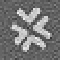
\includegraphics[height=\heightof{M}]{autanet.pdf}}
\definecolor{mygray}{gray}{0.333}
\iftypodisclaim%
\ifafour\newcommand\addprintnote{\begin{picture}(0,0)%
\put(245,149){\makebox(0,0){\rotatebox{90}{\tiny\color{mygray}\textsf{This
            document is designed for screen reading and
            two-up printing on A4 or Letter paper}}}}%
\end{picture}}% A4
\else\newcommand\addprintnote{\begin{picture}(0,0)%
\put(176,112){\makebox(0,0){\rotatebox{90}{\tiny\color{mygray}\textsf{This
            document is designed for screen reading and
            two-up printing on A4 or Letter paper}}}}%
\end{picture}}\fi%afourtrue
\makeoddfoot{plain}{}{\makebox[0pt]{\thepage}\addprintnote}{}
\else
\makeoddfoot{plain}{}{\makebox[0pt]{\thepage}}{}
\fi%typodisclaimtrue
\makeoddhead{plain}{}{}{\footnotesize\reporthead}

% \copypagestyle{manainitial}{plain}
% \makeheadrule{manainitial}{\headwidth}{0.5\normalrulethickness}
% \makeoddhead{manainitial}{%
% \footnotesize\sffamily%
% \scshape\headauthor}{}{\footnotesize\sffamily%
% \headtitle}
% \makeoddfoot{manaart}{}{\thepage}{}

\pagestyle{manaart}

\setlength{\droptitle}{-3.9\onelineskip}
\pretitle{\begin{center}\LARGE\sffamily%
\bfseries}
\posttitle{\bigskip\end{center}}

\makeatletter\newcommand*{\atf}{
\includegraphics[%trim=1pt 1pt 0pt 0pt,
totalheight=\heightof{@}]{atblack.png}}\makeatother
\providecommand{\affiliation}[1]{\textsl{\textsf{\footnotesize #1}}}
\providecommand{\epost}[1]{\texttt{\footnotesize\textless#1\textgreater}}
\providecommand{\email}[2]{\href{mailto:#1ZZ@#2 ((remove ZZ))}{#1\protect\atf#2}}

\preauthor{\vspace{-0.5\baselineskip}\begin{center}
\normalsize\sffamily%
\lineskip  0.5em}
\postauthor{\par\end{center}}
\predate{\DTMsetdatestyle{mydate}\begin{center}\footnotesize}
\postdate{\end{center}\vspace{-\medskipamount}}
\usepackage[british]{datetime2}
\DTMnewdatestyle{mydate}%
{% definitions
\renewcommand*{\DTMdisplaydate}[4]{%
\number##3\ \DTMenglishmonthname{##2} ##1}%
\renewcommand*{\DTMDisplaydate}{\DTMdisplaydate}%
}
\DTMsetdatestyle{mydate}


\setfloatadjustment{figure}{\footnotesize}
\captiondelim{\quad}
\captionnamefont{\footnotesize\sffamily%
}
\captiontitlefont{\footnotesize}
\firmlists*
\midsloppy

% handling orphan/widow lines:
\clubpenalty=10000
\widowpenalty=10000
\raggedbottom

\selectlanguage{british}\frenchspacing
%%%%%%%%%%%%%%%%%%%%%%%%%%%%%%%%%%%%%%%%%%%%%%%%%%%%%%%%%%%%%%%%%%%%%%%%%%%%
%%%%%%%%%%%%%%%%%%%%%%%%%%%%%%%%%%%%%%%%%%%%%%%%%%%%%%%%%%%%%%%%%%%%%%%%%%%%
%%%% Paper's details %%%%
\title{\propertitle%\\
%  {\large A geometric commentary on maximum-entropy proofs}% ***
}
\author{\ifpublic\hspace*{\stretch{1}}%
%\begin{tabular}[t]{c}
\parbox[t]{0.3\linewidth}{\protect\centering%
Alex\\%
{\footnotesize\epost{\email{alsfilip}{mail.med.penn.edu}}}}%
%\end{tabular}&%
\hspace*{\stretch{1}}%
%\begin{tabular}[t]{c}
\parbox[t]{0.3\linewidth}{\protect\centering%
P.G.L. Porta\,Mana\\%
{\footnotesize%\ \href{https://orcid.org/0000-0002-6070-0784}{\protect\includegraphics[scale=0.16]{orcid_32x32.png}}}\\{\footnotesize
\epost{\email{pgl}{portamana.org}}}%
}% \\%
% {\footnotesize\href{https://orcid.org/0000-0002-6070-0784}{\protect\includegraphics[scale=0.16]{orcid_32x32.png}\textsc{orcid}:0000-0002-6070-0784}}%
%\end{tabular}%
\hspace*{\stretch{1}}%
\else Alex, Luca, Yasser, \etal%
\fi}

\date{Draft of \today\ (first drafted \firstdraft)}
%\date{\firstpublished; updated \oggi}

%@@@@@@@@@@ new macros @@@@@@@@@@
% Common ones - uncomment as needed
%\providecommand{\nequiv}{\not\equiv}
%\providecommand{\coloneqq}{\mathrel{\mathop:}=}
%\providecommand{\eqqcolon}{=\mathrel{\mathop:}}
%\providecommand{\varprod}{\prod}
\newcommand*{\de}{\partialup}%partial diff
\newcommand*{\pu}{\piup}%constant pi
\newcommand*{\delt}{\deltaup}%Kronecker, Dirac
%\newcommand*{\eps}{\varepsilonup}%Levi-Civita, Heaviside
%\newcommand*{\riem}{\zetaup}%Riemann zeta
%\providecommand{\degree}{\textdegree}% degree
%\newcommand*{\celsius}{\textcelsius}% degree Celsius
%\newcommand*{\micro}{\textmu}% degree Celsius
%\newcommand*{\I}{\mathrm{i}}%imaginary unit
%\newcommand*{\e}{\mathrm{e}}%Neper
\newcommand*{\di}{\mathrm{d}}%differential
%\newcommand*{\Di}{\mathrm{D}}%capital differential
%\newcommand*{\planckc}{\hslash}
%\newcommand*{\avogn}{N_{\textrm{A}}}
%\newcommand*{\NN}{\bm{\mathrm{N}}}
%\newcommand*{\ZZ}{\bm{\mathrm{Z}}}
%\newcommand*{\QQ}{\bm{\mathrm{Q}}}
\newcommand*{\RR}{\bm{\mathrm{R}}}
%\newcommand*{\CC}{\bm{\mathrm{C}}}
%\newcommand*{\nabl}{\bm{\nabla}}%nabla
%\DeclareMathOperator{\lb}{lb}%base 2 log
%\DeclareMathOperator{\tr}{tr}%trace
%\DeclareMathOperator{\card}{card}%cardinality
%\DeclareMathOperator{\im}{Im}%im part
%\DeclareMathOperator{\re}{Re}%re part
%\DeclareMathOperator{\sgn}{sgn}%signum
%\DeclareMathOperator{\ent}{ent}%integer less or equal to
%\DeclareMathOperator{\Ord}{O}%same order as
%\DeclareMathOperator{\ord}{o}%lower order than
%\newcommand*{\incr}{\triangle}%finite increment
\newcommand*{\defd}{\coloneqq}
\newcommand*{\defs}{\eqqcolon}
%\newcommand*{\Land}{\bigwedge}
%\newcommand*{\Lor}{\bigvee}
%\newcommand*{\lland}{\mathbin{\ \land\ }}
%\newcommand*{\llor}{\mathbin{\ \lor\ }}
%\newcommand*{\lonlyif}{\mathbin{\Rightarrow}}%implies
%\newcommand*{\limplies}{\mathbin{\Rightarrow}}%implies
\newcommand*{\mimplies}{\Rightarrow}%implies
%\newcommand*{\liff}{\mathbin{\Leftrightarrow}}%if and only if
%\newcommand*{\cond}{\mathpunct{|}}%conditional sign (in probabilities)
%\newcommand*{\lcond}{\mathpunct{|\ }}%conditional sign (in probabilities)
%\newcommand*{\bigcond}{\mathpunct{\big|}}%conditional sign (in probabilities)
%\newcommand*{\lbigcond}{\mathpunct{\big|\ }}%conditional sign (in probabilities)
\newcommand*{\suchthat}{\mid}%{\mathpunct{|}}%such that (eg in sets)
%\newcommand*{\bigst}{\mathpunct{\big|}}%such that (eg in sets)
%\newcommand*{\with}{\colon}%with (list of indices)
%\newcommand*{\mul}{\times}%multiplication
%\newcommand*{\inn}{\cdot}%inner product
%\newcommand*{\dotv}{\mathord{\,\cdot\,}}%variable place
%\newcommand*{\comp}{\circ}%composition of functions
%\newcommand*{\con}{\mathbin{:}}%scal prod of tensors
%\newcommand*{\equi}{\sim}%equivalent to 
\renewcommand*{\asymp}{\simeq}%equivalent to 
%\newcommand*{\corr}{\mathrel{\hat{=}}}%corresponds to
%\providecommand{\varparallel}{\ensuremath{\mathbin{/\mkern-7mu/}}}%parallel (tentative symbol)
\renewcommand{\le}{\leqslant}%less or equal
\renewcommand{\ge}{\geqslant}%greater or equal
%\DeclarePairedDelimiter\clcl{[}{]}
\DeclarePairedDelimiter\clop{[}{[}
%\DeclarePairedDelimiter\opcl{]}{]}
%\DeclarePairedDelimiter\opop{]}{[}
%\DeclarePairedDelimiter\abs{\lvert}{\rvert}
%\DeclarePairedDelimiter\norm{\lVert}{\rVert}
\DeclarePairedDelimiter\set{\{}{\}}
%\DeclareMathOperator{\pr}{P}%probability
\newcommand*{\pf}{\mathrm{p}}%probability
\newcommand*{\p}{\mathrm{P}}%probability
%\newcommand*{\tf}{\mathrm{T}}%probability
\renewcommand*{\|}{\mathpunct{|}}
%\newcommand*{\lcond}{\mathpunct{|\ }}%conditional sign (in probabilities)
\newcommand*{\bigcond}{\mathpunct{\big|\ }}%conditional sign (in probabilities)
%\newcommand*{\lbigcond}{\mathpunct{\big|\ }}%conditional sign (in probabilities)
%\newcommand*{\+}{\lor}
%\renewcommand{\*}{\land}
\newcommand*{\sect}{\S}% Sect.~
\newcommand*{\sects}{\S\S}% Sect.~
\newcommand*{\chap}{ch.}%
\newcommand*{\chaps}{chs}%
\newcommand*{\bref}{ref.}%
\newcommand*{\brefs}{refs}%
%\newcommand*{\fn}{fn}%
\newcommand*{\eqn}{eq.}%
\newcommand*{\eqns}{eqs}%
\newcommand*{\fig}{fig.}%
\newcommand*{\figs}{figs}%
\newcommand*{\vs}{{vs.}}
\newcommand*{\etc}{{etc.}}
\newcommand*{\ie}{{i.e.}}
%\newcommand*{\ca}{{c.}}
\newcommand*{\eg}{{e.g.}}
\newcommand*{\foll}{{ff.}}
%\newcommand*{\viz}{{viz}}
\newcommand*{\cf}{{cf.}}
%\newcommand*{\Cf}{{Cf.}}
%\newcommand*{\vd}{{v.}}
%\newcommand*{\etsim}{{et sim.}}
%\newcommand*{\ibid}{{ibid.}}
%\newcommand*{\sic}{{sic}}
%\newcommand*{\id}{\mathte{I}}%id matrix
%\newcommand*{\nbd}{\nobreakdash}%
%\newcommand*{\bd}{\hspace{0pt}}%
%\def\hy{-\penalty0\hskip0pt\relax}
%\newcommand*{\labelbis}[1]{\tag*{(\ref{#1})$_\text{r}$}}
%\newcommand*{\mathbox}[2][.8]{\parbox[t]{#1\columnwidth}{#2}}
%\newcommand*{\zerob}[1]{\makebox[0pt][l]{#1}}
\newcommand*{\tprod}{\mathop{\textstyle\prod}\nolimits}
\newcommand*{\tsum}{\mathop{\textstyle\sum}\nolimits}
%\newcommand*{\tint}{\begingroup\textstyle\int\endgroup\nolimits}
%\newcommand*{\tland}{\mathop{\textstyle\bigwedge}\nolimits}
%\newcommand*{\tlor}{\mathop{\textstyle\bigvee}\nolimits}
%\newcommand*{\sprod}{\mathop{\textstyle\prod}}
%\newcommand*{\ssum}{\mathop{\textstyle\sum}}
%\newcommand*{\sint}{\begingroup\textstyle\int\endgroup}
%\newcommand*{\sland}{\mathop{\textstyle\bigwedge}}
%\newcommand*{\slor}{\mathop{\textstyle\bigvee}}
%\newcommand*{\T}{^\intercal}%transpose
%\newcommand*{\E}{\mathrm{E}}
%\DeclarePairedDelimiter\expp{(}{)}
%\newcommand*{\expe}{\E\expp}%round
%\newcommand*{\expeb}{\E\clcl}%square
%%\newcommand*{\QEM}%{\textnormal{$\Box$}}%{\ding{167}}
%\newcommand*{\qem}{\leavevmode\unskip\penalty9999 \hbox{}\nobreak\hfill
%\quad\hbox{\QEM}}

\definecolor{notecolour}{RGB}{68,170,153}
%\newcommand*{\puzzle}{{\fontencoding{U}\fontfamily{fontawesometwo}\selectfont\symbol{225}}}
\newcommand*{\puzzle}{\maltese}
\newcommand{\mynote}[1]{ {\color{notecolour}\puzzle\ #1\ }}
%\newcommand*{\widebar}[1]{{\mkern1.5mu\skew{2}\overline{\mkern-1.5mu#1\mkern-1.5mu}\mkern 1.5mu}}

%\DeclareMathOperator*{\argsup}{arg\,sup}
\newcommand*{\ptext}[1]{\text{\small #1}}
\newcommand*{\simpl}{\varDelta}
\newcommand*{\yqq}{q}
\newcommand*{\yq}{\bm{\yqq}}
\newcommand*{\yff}{f}
\newcommand*{\yf}{\bm{\yff}}
\newcommand*{\yMJ}{M_{\text{J}}}
\newcommand*{\yN}{\varLambda}
\newcommand*{\ynn}{\nu}
\newcommand*{\yn}{\bm{\nu}}
\newcommand*{\yth}{\theta}
\newcommand*{\yTh}{\varTheta}
\newcommand*{\ymu}{\mu}
\newcommand*{\yh}{\chi}
\newcommand*{\yI}{I}
\newcommand*{\yrs}{h}
\AtBeginEnvironment{tabularx}{\setlist[enumerate]{wide, leftmargin=*,
    itemsep=0pt%, before=\vspace{-\dimexpr\baselineskip +2 \partopsep},
    % after=\vspace{-\baselineskip}
  }}
%@@@@@@@@@@ new macros end @@@@@@@@@@

\firmlists
\begin{document}
\captiondelim{\quad}\captionnamefont{\footnotesize}\captiontitlefont{\footnotesize}
\selectlanguage{british}\frenchspacing

%%% Title and abstract %%%
\maketitle
\ifpublic
\abstractrunin
\abslabeldelim{}
\renewcommand*{\abstractname}{}
\setlength{\absleftindent}{0pt}
\setlength{\absrightindent}{0pt}
\setlength{\abstitleskip}{-\absparindent}
\begin{abstract}\labelsep 0pt%
  \noindent How does a Bayesian robot do at Plinko, using an infinitely
  exchangeable model and borrowing a human participant's prior?
% \par%\\[\jot]
% \noindent
% {\footnotesize PACS: ***}\qquad%
% {\footnotesize MSC: ***}%
%\qquad{\footnotesize Keywords: ***}
\end{abstract}\fi

\selectlanguage{british}\frenchspacing
% \asudedication{\small ***}
% \vspace{\bigskipamount}

% \setlength{\epigraphwidth}{.7\columnwidth}
% \setlength{\epigraphrule}{0pt}
% \epigraphfontsize{\footnotesize}%
\setlength{\epigraphwidth}{.6\columnwidth}
%\epigraphposition{flushright}
\epigraphtextposition{flushright}
%\epigraphsourceposition{flushright}
\epigraphfontsize{\footnotesize}
\setlength{\epigraphrule}{0pt}
\setlength{\beforeepigraphskip}{0pt}
\setlength{\afterepigraphskip}{0pt}
\epigraph{We are human, after all\\
  Much in common, after all}{\citep{daftpunk2005b}}
%\vspace{-1em}
% \epigraph{If people always felt obliged to back their opinions when
%   challenged, we would be spared a few of the ``certain'' predictions that
%   are so freely made.}{\citep{good1950}}


% \noindent\emph{\footnotesize Note: Dear Peer, this manuscript is
%   peer-reviewed by \emph{you}. I'm grateful if you let me know of any
%   faults in its premisses, logic, evidence, and of any other criticisms you
%   may have.}


\section{Remarks, comments, thoughts on the project}
\label{sec:method_remarks}

\subsection{[Luca] What goes on in a participant's head? Possible models}

The experimental setup is open to a huge number of analyses and
interpretations on the participants' part, inspired by past experience. As
participants we can surmise that there's a connection between different
trials, some sort of \enquote{constant mechanism} at some level. Or we can
surmise that there's no such connection, hence observation of past trials
doesn't say anything about the next one. Or we can surmise that the next
trial is influenced by the participant's own bar-height assignments. And
many other hypotheses. We can also entertain all these hypotheses at the
same time, and shift from one to another during the experiment. For
example, if we suddenly wondered whether the computer program is actually
using our bar distribution, we could suddenly move all probability to a
slot at the edge and check if this seems to influence the next outcome
(\cf\ participant~31).

The same goes for the choice of initial distribution. As
participants we can say \enquote{alright, there are 40 slots}, and just
give a uniform distributions to the 40 possibilities. Or we can consider
the pyramidal mechanism of the game, which leads to a binomial
distribution. Or we can consider that this is a computerized version of the
game. The computer could simulate the physics of the actual game; but the
image of the mechanism could also be just for show, the computer being
programmed to distribute the outcomes according to a predetermined,
completely arbitrary distribution. From this point of view we could again
decide to assign a uniform distribution.

\subsection{[Luca] Paradigms for judgement and assessment}

The literature I've seen so far explains at length how the data presented
to participants are generated, and is very succinct in explaining what was
said to the participants before the experiment. The participant's behaviour
is the compared against models based on the pseudo-random algorithm that
generated the data. Nassar \etal's \citey{nassaretal2010} work is an
example.

I think that we should use a different paradigm to describe the experiment
and assess the participants' behaviours.

As I see it, the participants' inferential behaviours should be compared
with that of a \enquote{robot} that uses exact or approximate Bayesian or
decision-theoretic rules, and that \emph{starts from the same information
  that was given to the participants}. So it's really important that this
information be explained at length, and whatever the participants were told
should be reported verbatim.

I don't see the rationale of comparing a participant who doesn't know the
data-generating algorithm, with a robot that does. Such a robot is
modelling a different initial state of knowledge. What's important here,
instead, is to model the inference, given the same initial knowledge.

A consequence of this point of view is that there isn't just one robot that
can model the inferences. The information given to the participants is
never be enough to make numeric inferences and apply the probability
calculus: it must always be augmented with additional assumptions,
determined by each participant's previous life experiences. Different
robots can thus be constructed: they use the same initial information as
the participants, but each is augmented with different auxiliary
assumptions. \emph{The} ideal observer doesn't exist. There are several
ideal observers.

Another consequence of this point of view is that the data-generating
algorithm becomes slightly less important. The robot is constructed based
on the exact information given the participants, and uses the same data
given to the participants. The data-generating algorithm nowhere enters in
the construction of the robot.

\iffalse
De~Finetti introduced the notion of exchangeability in order to avoid
thinking in terms of \enquote{mechanisms} or of \enquote{true unknown
  distributions} \citep[\cf][\chap~3]{good1965}. He characterized a
statistical model in terms of \emph{features of the predictive
  distribution} -- for example, that it be invariant under exchanges of the
outcomes. This point of view was taken up by many other statisticians and
has been used to characterize many other statistical models, like Markov
ones for example
\citep{freedman1962,diaconisetal1980c,zaman1984,fortinietal2002,fortinietal2014}.
\fi


\section{First study: exchangeable-model robot}
\label{sec:first_study}

\subsection{The Bayesian robot}
\label{sec:bayes_robot}

In the context of these notes and of the Plinko experiments
\citep{filipowiczetal2014,filipowiczetal2016} we call \enquote{model} any
set of assumptions that allows us to assign a probability to a new
observation, given a number of observations of a similar kind. Denote such
assumptions by a proposition $M$ -- a proposition surely very difficult to
express in writing. Denote the proposition \enquote{The outcome of the
  $i$th observation is $d$} by $D_{d}^i$, with $d \in \set{1,\dotsc N}$.
Then $M$ allows us to give a numeric value to
\begin{equation}
  \label{eq:general_prediction}
  \p(D^{m+1}_{d_{m+1}} \|
  D^m_{d_m} \land \dotsb \land  D^2_{d_2} \land D^1_{d_1} \land  M),
\end{equation}

We will abbreviate logical conjunction \enquote{$\land$} with a comma, for
simplicity. Our statistical terminology and notation follow ISO standards
\citep{iso1993_r2009,iso2006} otherwise.

We shall consider a robot who uses either of these two equivalent
assumptions:
\begin{itemize}
\item the joint distribution for any number of observations is symmetric with
respect to their order; that is, the order of the observations is
irrelevant for inferential purposes;
\item for inferential purposes, only the relative frequencies of past observations
  are relevant. Any additional data about past observation is irrelevant
  and can be discarded.
\end{itemize}
Distributions for different number of observations must of course be
consistent with one another through marginalization.

The two equivalent assumptions are technically called \emph{infinite
  exchangeability}. This notion was introduced by de~Finetti
\parentext{\cite*{definetti1930,definetti1937}; \cite{heathetal1976}}; it
is described in detail in \textcite[\sect~4.2]{bernardoetal1994_r2000}.

Infinite exchangeability determines this form of the probability above:
\begin{equation}
  \label{eq:exchangeability_form}
  \p(D^1_{d_1} , D^2_{d_2} , \dotsc , D^m_{d_m} \| M) =
  \int_\simpl   \Biggl( \prod_{i=1}^m \yqq_{d_i} \Biggr)\, \pf(\yq \| M)\,\di\yq,
\end{equation}
where $\yq$ is a normalized $N$-tuple of positive numbers:
$\simpl \defd \set{\yq \in \RR^N \suchthat \yqq_i\ge0,
  \sum_{i=1}^N\yqq_i=1}$. This $N$-tuple can be thought of the relative,
long-run frequencies of the possible outcomes\footnote{\enquote{But this
    \emph{long run} is a misleading guide to current affairs. \emph{In the
      long run} we are all dead.} \citep[\sect~3.I,
  p.~65]{keynes1923_r2013}}, and $\pf(\yq \| M)\,\di\yq$ as their
probability density. From this point of view it is as if the robot first
assumes to know the long-run frequencies of the different outcomes and, not
knowing their particular order in the observation, 
assigns to the occurrence of each a probability proportional to its
frequency: this is the term $\prod_{i=1}^m \yqq_{d_i}$ in the integral.
Then, not being sure about the long-run frequencies, the robot assign to
them the density $\pf(\yq \| M)\,\di\yq$ -- which is determined by
additional assumptions besides exchangeability.

As an explicit example, say with $N=40$,
\begin{equation}
  \label{eq:exchangeability_form_example}
  \p(D^1_{37} , D^2_{6} , D^3_{25}, D^4_{37} \| M) =
  \int_\simpl \yqq_{6}\, \yqq_{25} \, {\yqq_{37}}^2\;  \pf(\yq \| M)\,\di\yq.
\end{equation}
In the following we omit the integration domain $\simpl$.

From Bayes's theorem we obtain the expression for the predictive
probability~\eqref{eq:general_prediction} of an infinite exchangeable model:
\begin{subequations}\label{eq:prediction_exchangeability}
  \begin{gather}
    \p(D^{m+1}_{d_{m+1}}\| D^1_{d_1}, \dotsc , D^m_{d_m} , M)
    = \int \yqq_{d_{m+1}} \pf(\yq \| D^1_{d_1}, \dotsc, D^m_{d_m}, M)\,\di\yq,
    \\
    \pf(\yq \| D^1_{d_1}, \dotsc, D^m_{d_m}, M)
    = \frac{ \bigl( \prod_{i=1}^m \yqq_{d_i} \bigr)\, \pf(\yq \| M)
      }{
      \int  \bigl( \prod_{i=1}^m \yqq_{d_i}' \bigr)\, \pf(\yq' \| M)\,\di\yq'
      }.
\label{eq:exchang_updated_prior}
  \end{gather}
\end{subequations}
Continuing our numeric example~\eqref{eq:exchangeability_form_example} this
could be
\begin{subequations}\label{eq:prediction_exchangeability_example}
  \begin{gather}
    \begin{multlined}[][0.95\linewidth]
    \p(D^5_{6} \| D^1_{37} , D^2_{6} , D^3_{25}, D^4_{3}, M)
    ={}\\ \int \yqq_{6}\; \pf(\yq \|  D^1_{37} , D^2_{6} , D^3_{25}, D^4_{3}, M)\,\di\yq,
  \end{multlined}
    \\
    \pf(\yq \|  D^1_{37} , D^2_{6} , D^3_{25}, D^4_{3}, M)
    = \frac{ \yqq_{6}\, \yqq_{25} \, {\yqq_{37}}^2\; \pf(\yq \| M)
      }{
      \int \yqq_{6}\, \yqq_{25} \, {\yqq_{37}}^2\; \pf(\yq' \| M)\,\di\yq'
      }.
  \end{gather}
\end{subequations}


Formula~\eqref{eq:prediction_exchangeability} tell us how our robot would
update its predictive probabilities at each new observation of a Plinko outcome.
\textcolor{white}{If you find this you can claim a postcard from me.}
%


\subsection{General remarks on the robot's behaviour}
\label{sec:remarks}

The exchangeable-model formula~\eqref{eq:prediction_exchangeability} leads
to some characteristic features of the robot's beliefs and of their
evolution:
\begin{itemize}
\item The robot's predictions can be interpreted in several ways. One is
  this: the robot believes that there's \enquote{something} constant in all
  trials; loosely speaking, a \enquote{constant mechanism}. Another, maybe
  preferable, is this: the robot has memory of past observations, but not
  of their order; any trends are therefore invisible to it.
\item As data accumulate, the robot's probabilities for the next outcome
  approach the observed frequencies. Such approach happens independently of
  the form of the prior $\pf(\yq \| M)\,\di\yq$ -- unless the latter is
  zero in peculiar regions of the integration domain -- but the prior
  determines the celerity of the approach. A prior heavily peaked on a
  frequency $\yq'$ will require a lot of data to move the predictions to
  a very different frequency $\yq$.
\item As data $D$ accumulate, the updated density
  $\pf(\yq \| D, M)\,\di\yq$ will become more and more peaked at the
  $N$-tuple of observed frequencies.
\item Suppose that we first have a long sequence of observations
  concentrating around frequencies $\yq$ -- say, a very long sequence of
  $1$s in a row -- and then a shift to other frequencies $\yq'$ -- say,
  suddenly $2$s only appear. After the shift, the predictive probabilities
  will eventually become peaked around the new frequencies, but the shift
  in the peaks will take a larger number of observations around the new
  frequencies than the number around the old frequencies.
\end{itemize}


\subsection{Initial prior}
\label{sec:initial_prior}

The shape of the initial prior heavily determines the predictions in the
first observations, so it must be chosen with care. The Plinko data tell us
the initial predictive probabilities of the participants,
\begin{equation}
  \label{eq:initial_predictive}
  \pf(D^1_{k} \| M) \equiv \int \yqq_{k}\; \pf(\yq \| M)\,\di\yq,
\end{equation}
but not their prior $\pf(\yq \| M)\,\di\yq$.

As a first study we consider a \emph{Johnson-Dirichlet} prior,
proportional to a monomial $\prod_i{\yq_i}^{x_i}$ for some values of $x_i$:
\begin{equation}
  \label{eq:JD_prior}
  \pf(\yq \| \yMJ) =
  \frac{\Gamma(\yN)}{\prod_i \Gamma(\yN\ynn_i)}\,
  \prod_{i=1}^N{\yq_i}^{\yN\ynn_i-1}, \qquad \yN>0, \ynn \in \simpl.
\end{equation}

This prior is determined by the additional assumption -- call it $\yMJ$ --
that that the frequencies of other outcomes are irrelevant for predicting a
particular one:
\begin{equation}
  \label{eq:sufficientness}
  \p(D^{m+1}_k \| N\yf, \yMJ) = \p(D^{m+1}_k \| N\yff_{k}, \yMJ)
  \qquad k\in\set{1,\dotsc, N},
\end{equation}
where $\yf$ is the $N$-tuple of observed relative frequencies. This
assumption is called \enquote{sufficientness}
\cites{johnson1924,johnson1932c}[\chap~4]{good1965}{zabell1982,jaynes1986d_r1996}.
% Asymptotically it leads \citep{jaynes1986d_r1996,portamana2009} to a
% predictive distribution of a maximum-entropy with Burg's \citey{burg1975} entropy
% $\tsum\ln\yx$.
This is a conjugate prior
\cites[\chap~9]{degroot1970_r2004}{diaconisetal1979b} and it has two convenient
properties: it updates to a density of the same mathematical form, and its
corresponding predictive distribution can be calculated analytically using
the formula
\begin{equation}
  \label{eq:Dirichlet_formula}
  \int_{\simpl} \prod_{i=1}^N {\yqq_{i}}^{x_i-1}\,\di\yq = \frac{\prod_i \Gamma(x_i)}{\Gamma\bigl(\sum_i x_i\bigr)}.
\end{equation}

We obtain for the initial distribution:
\begin{equation}
  \label{eq:initial_predictive_JD}
  \p(D^1_{k} \| \yMJ) = \int \yqq_{k}\; \pf(\yq \| \yMJ)\,\di\yq
  = \ynn_k,
\end{equation}
and for the updated density:
\begin{multline}
  \label{eq:update_prior_JD}
  \pf(\yq \| D^1_{d_1}, \dotsc, D^m_{d_m}, \yMJ)
  = 
  \frac{\Gamma(\yN')}{\prod_i \Gamma(\yN'\ynn_i')}\,
  \prod_{i=1}^N{\yq_i}^{\yN'\ynn_i'-1}
  \\\
  \text{with}\quad \yN' =\yN+N,\quad
  \yn'=\frac{\yN\yn+N\yf}{\yN+N}.
\end{multline}

Formula~\eqref{eq:initial_predictive_JD} says that the Johnson-Dirichlet
prior can produce any initial probabilities assigned by the participants,
just by equalling the parameters $\yn$ to them. The parameter $\yN$ is left
arbitrary. We can call it the \emph{stubbornness} of the robot, Here's the reason.

Suppose that after some observations the predictive distribution is $\yn$,
and that the next outcome is $k$. Then the probability distribution for the
slots is updated to:
\begin{multline}
  \label{eq:predictive_JD}
  \p(D^{m+1}_{j} \| D^{m}_{k}, \yn^{m},\yN^{m}, \yMJ) =
  \ynn^{m+1}_j \defd
  \frac{\yN^{m}}{\yN^{m}+1}\ynn^{m}_j +
    \begin{dcases}
      \frac{1}{\yN^{m}+1} &\text{if $j=k$},
      \\[2\jot]
      0 &\text{if $j\ne k$},
    \end{dcases}
    \\[2\jot]
    \text{and $\yN^{m+1} \defd \yN^{m}+1$}.
\end{multline}
This update corresponds to a participant's raising the bar assignment under
slot $k$, leaving the others untouched, and/or lowering the bar assignments
for \emph{all} other slots by the same proportion. The parameter $\yN$ is
increased by $1$. The larger $\yN$, the more reluctant the robot is in
revising its guesses in the light of new observations. The update
formula~\eqref{eq:update_prior_JD} says that the robot behaves as if it had
already made $\yN$ observations with outcome frequencies $\yn$.



\subsection{Examples: participant vs robot}
\label{sec:examples_partic_robot}

Let's choose a participant, and use
formula~\eqref{eq:initial_predictive_JD} to choose the $\yn$ parameters of
the robot's prior, equating it to the initial predictive distribution of
the participant. Let's set a value for the robot's stubbornness $\yN$, and
check how the robot updates its predictive distribution, using
formula~\eqref{eq:update_prior_JD}, while observing the same outcomes as
the participant.


\begin{figure}[p!]
\centering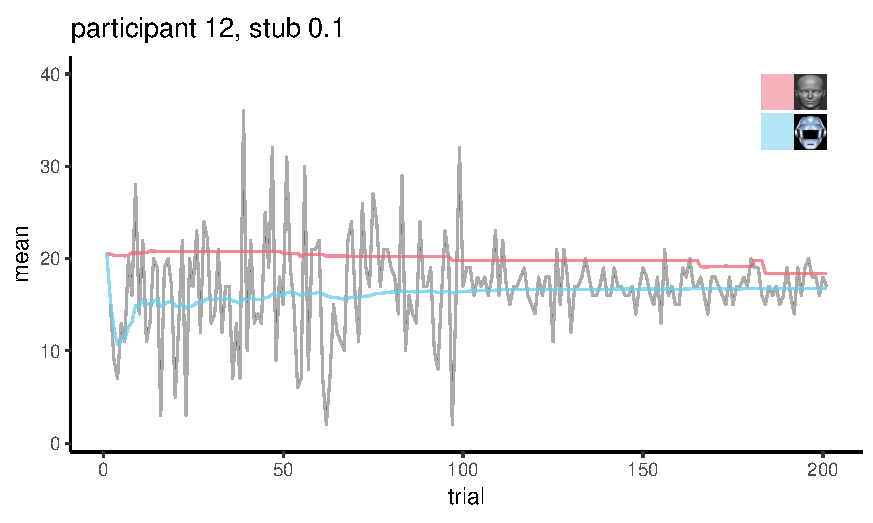
\includegraphics[width=\linewidth]{{comparisons1/means_12-stub_0.1}.pdf}
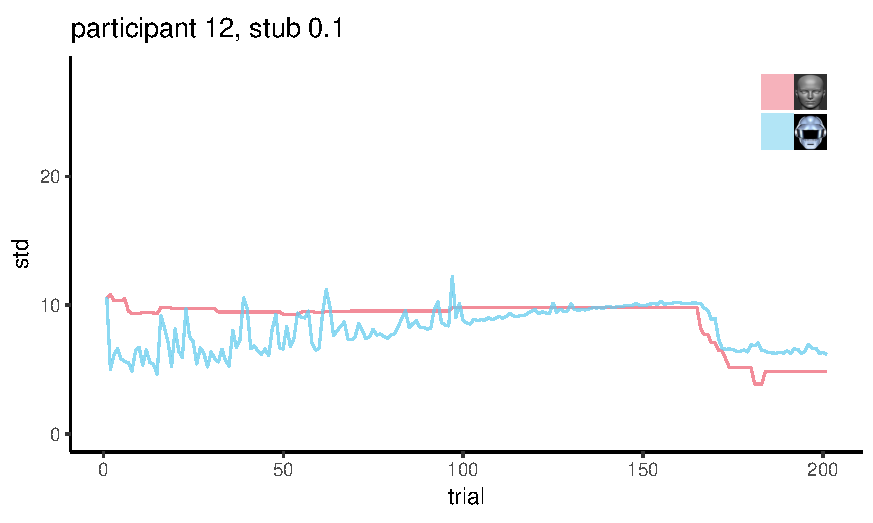
\includegraphics[width=\linewidth]{{comparisons1/stds_12-stub_0.1}.pdf}
\caption{Comparison of the means and standard deviations of the predictive
  distributions of participant~12 and of a robot with stubborness
  $\yN=0.1$}\label{fig:comparison_12_01}
\end{figure}% done with exploration1.R
Figure~\ref{fig:comparison_12_01} shows the means and standard deviations
of the sequence such predictive distributions, for participant~12 and a
robot with stubbornness $\yN=0.1$. This low value makes the robot give
great consideration to the first outcomes, as the initial variability in
the figure shows. The program generating the outcomes had a change in
standard deviation, shifting to a narrower distribution at trial~101. The
robot adapted to this change very slowly.


\begin{figure}[p!]
\centering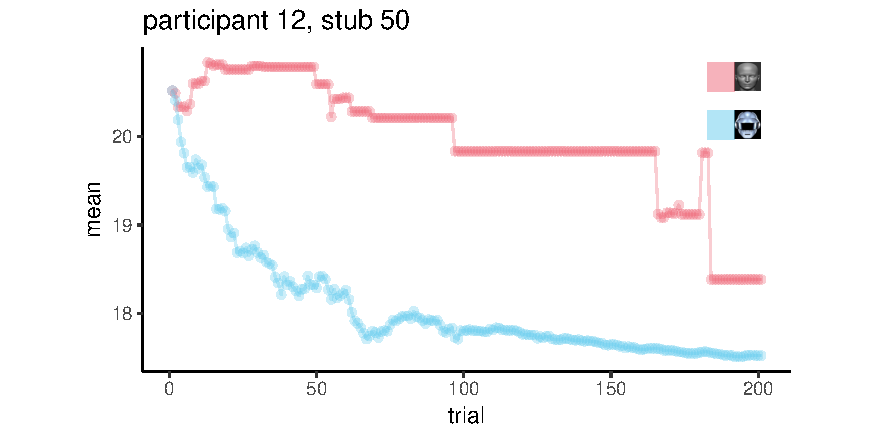
\includegraphics[width=\linewidth]{{comparisons1/means_12-stub_50}.pdf}
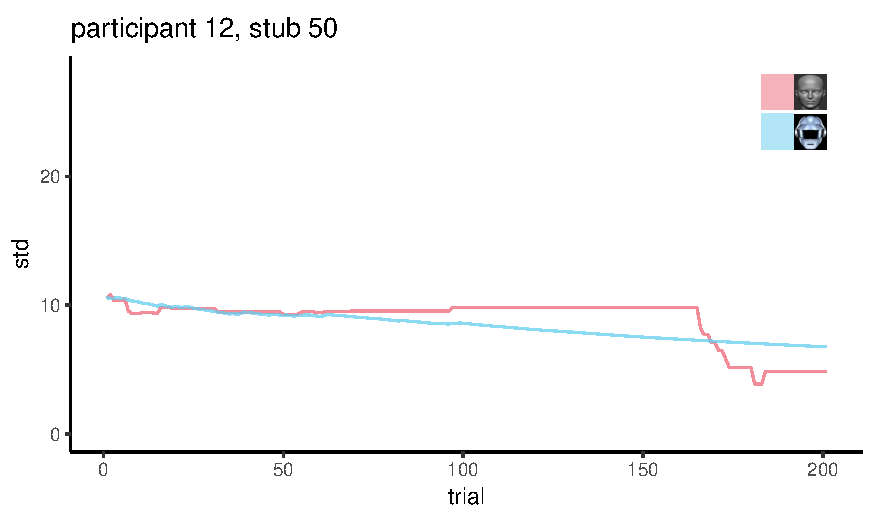
\includegraphics[width=\linewidth]{{comparisons1/stds_12-stub_50}.pdf}
\caption{Comparison of the means and standard deviations of the predictive
  distributions of participant~12 and of a robot with stubborness
  $\yN=50$}\label{fig:comparison_12_50}
\end{figure}% done with exploration1.R
Figure~\ref{fig:comparison_12_50} is analogous to
\fig~\ref{fig:comparison_12_01} but for a robot with stubbornness
$\yN=50$. This robot is even more slow to adapt to the narrowing in the
standard deviation of the generated outcomes.


\begin{figure}[p!]
\centering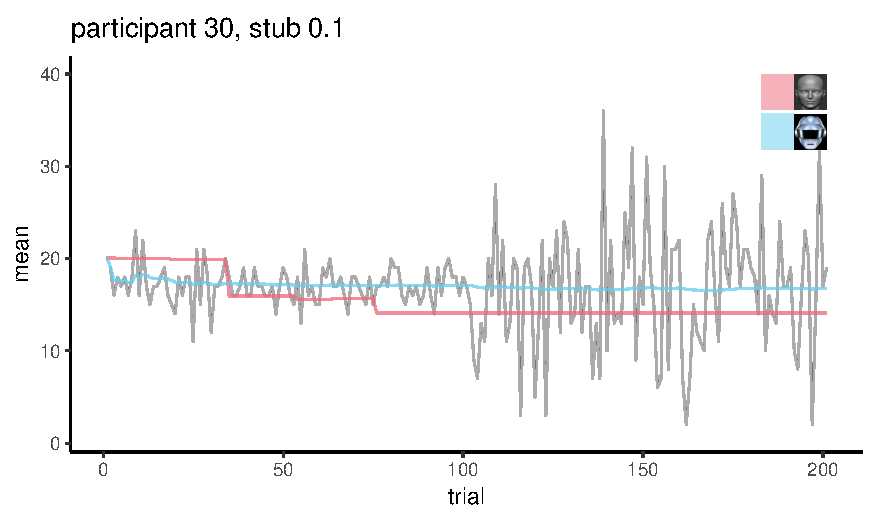
\includegraphics[width=\linewidth]{{comparisons1/means_30-stub_0.1}.pdf}
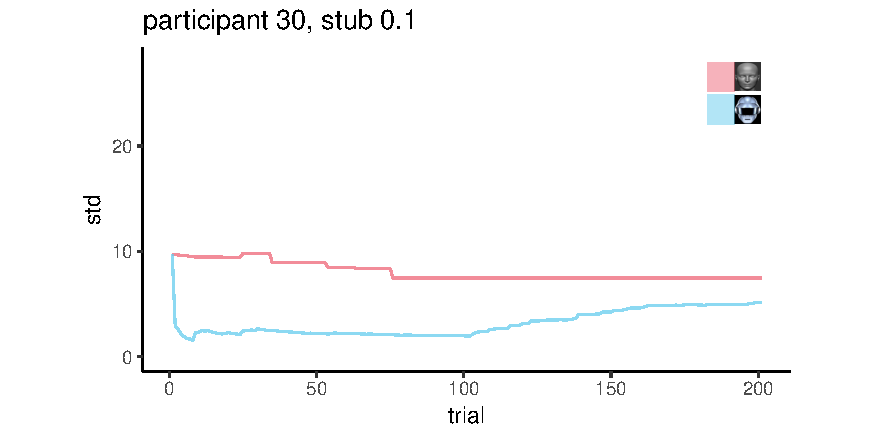
\includegraphics[width=\linewidth]{{comparisons1/stds_30-stub_0.1}.pdf}
\caption{Comparison of the means and standard deviations of the predictive
  distributions of participant~30 and of a robot with stubborness
  $\yN=0.1$}\label{fig:comparison_30_01}
\end{figure}% done with exploration1.R
\begin{figure}[p!]
\centering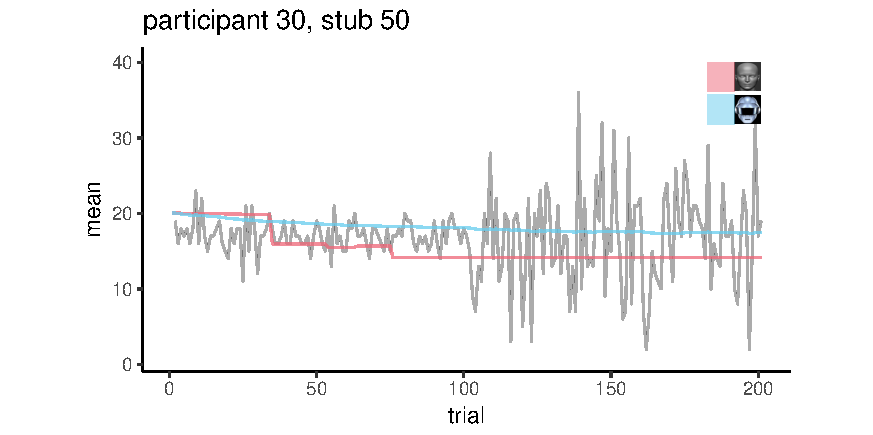
\includegraphics[width=\linewidth]{{comparisons1/means_30-stub_50}.pdf}
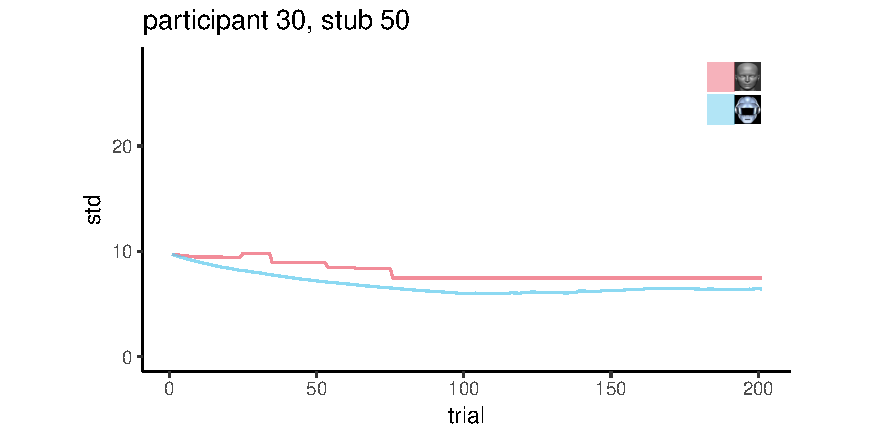
\includegraphics[width=\linewidth]{{comparisons1/stds_30-stub_50}.pdf}
\caption{Comparison of the means and standard deviations of the predictive
  distributions of participant~30 and of a robot with stubborness
  $\yN=50$}\label{fig:comparison_30_50}
\end{figure}% done with exploration1.R
Figures~\ref{fig:comparison_30_01} and~\ref{fig:comparison_30_50} show
the same for participant~30. The change in standard deviation was from
narrow to large in this case.

The robot with low stubbornness seems to adapt to the widening of the
outcome outputs faster than it had for the narrowing of the previous case:
the change in the slope of the robot's standard-deviation curve seems
steeper in \fig~\ref{fig:comparison_30_01} than
in~\ref{fig:comparison_12_01}.


If we look at the sequence of outcomes of \figs~\ref{fig:comparison_12_01}
or~\ref{fig:comparison_30_01}, we perceive that something changed around
trial~100. If we could plot these outcomes while they are generated, we
would likely notice the change by around trial~25. Our robot, however,
can't detect this change for the reasons explained in
\sect~\ref{sec:remarks}; any outcomes from narrow or wide generating
processes are mingled in the robot's memory.

Only non-exchangeable or hierarchic models can exhibit a short evidence
memory and be capable of believing that the underlying \enquote{mechanism}
has changed.


Some conclusions can be drawn from the properties of our model and from the
examples:
\begin{itemize}[para]
\item Participants who have great inertia against updating their
  predictions in view of the observations are \emph{not} necessarily
  behaving at variance with the probability calculus. The latter says that
  they can be as stubborn as they please: larger $\yN$. If we judge such
  inertia as irrational, our judgement cannot be based on such a simple
  model; possibly it's based on a hierarchic model where $\yN$ is given a
  probability that depends on past experiences.

\item The slots have a specific physical order, and from the way the ball
  falls into them it seems reasonable to assume that updates to the
  probability for one slot should affect those for nearby slots. The
  Johnson-Dirichlet model does not take this into account. 

\item A participant who, after observing outcome $k$, raises the bar under
  that slot \emph{and nearby bars} is therefore not acting according to a
  Johnson-Dirichlet exchangeable model.
\item Infinitely exchangeable priors are incapable of quickly adapting to
  changes in the empirical statistics of the outcomes.
\end{itemize}


\subsection{Robot's surprise}
\label{sec:examples_robot_surprise}

A robot with low stubbornness quickly adapts its predictions to the
observed outcomes, but as the outcomes accumulate its stubbornness
increases. If there is a late change in the generation of the outcomes, at
trial 101 for example, the robot will adapt its predictions more slowly.

It is interesting to ask: is this prediction adaptation the same for a
change from a narrow to a wide distribution, as for a change from a wide to
a narrow one? or is there a difference in the adaptation speed?

The answer depends on how we measure such speed. One way could be this:
starting from the trial in which the change occurs, we let a second robot
with low stubbornness observe the new outcomes and make predictions,
starting from frequency parameters equal to those reached by the first
robot. The second robot will quickly adapt to the new observed outcomes,
and we can use it as a touchstone for the first robot's adaptation speed.
The predictions of the second robot can also be interpreted as if we had
reset the stubbornness of the first robot to a low value.

\begin{figure}[b!]
\centering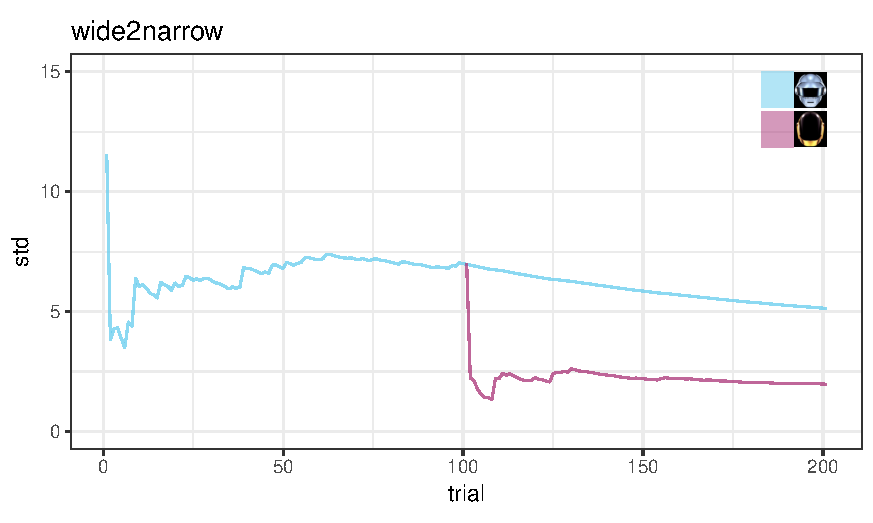
\includegraphics[width=\linewidth]{{comparisons1/compare_robots_wide2narrow-stub_0.1}.pdf}
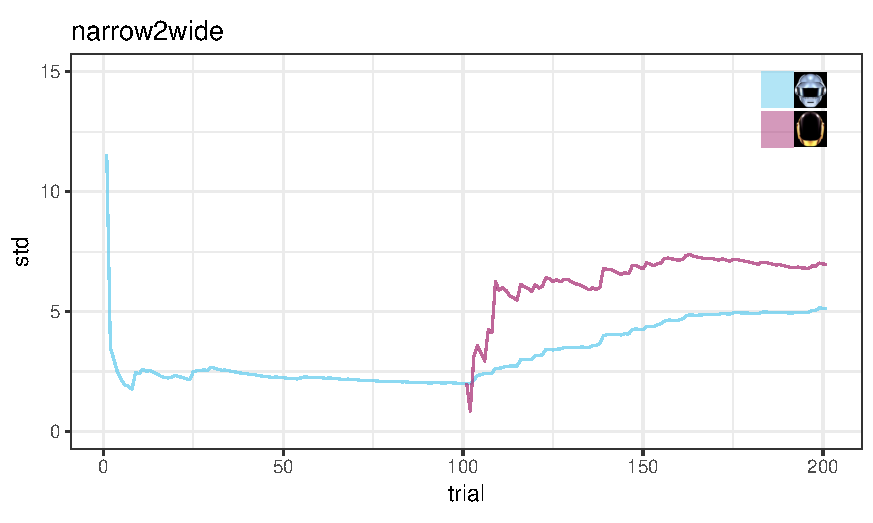
\includegraphics[width=\linewidth]{{comparisons1/compare_robots_narrow2wide-stub_0.1}.pdf}
\caption{Adaptation speed of the standard deviation for a robot after a
  change in the generation of the outcomes, compared with that of a robot
  that starts learning after the change. The final relative entropy for the
  first robot relative to the second is $1.01$ in the wide-to-narrow case,
  vs $0.260$ in the narrow-to-wide; exchanging the distributions: $0.283$
  vs $0.211$. The final normalized overlap is $0.949$ for wide-to-narrow vs
  $0.823$ for narrow-to-wide}\label{fig:comparison_robots_stds}
\end{figure}% done with exploration1.R
% wide2narrow: relentr=0.2825763, overlap=0.1059542
% narrow2wide: relentr=0.21082114, overlap=0.05119122
The results of this comparison are shown in
\fig~\ref{fig:comparison_robots_stds}. Looking at the standard deviations
of the distributions it seems that a robot adapts more slowly in going from
a wide to a narrow distribution than vice versa. This is true looking at
the final relative entropy of the first robot relative to the second:
$1.01$ wide-to-narrow vs $0.260$ narrow-to-wide; same if we exchange the
distributions: $0.283$ vs $0.211$. The overlap seems to say the
opposite: $0.106$ wide-to-narrow vs $0.0512$ narrow-to-wide; but the
overlap is heavily influenced by the narrowness of the overlapping
distributions, so it may not be a reliable measure in this case. If we use
the normalized overlap (corresponding to the cosine of the angle between
the distribution vectors) we find $0.949$ vs $0.823$, which agree with the
first three measures.

\begin{figure}[t!]
\centering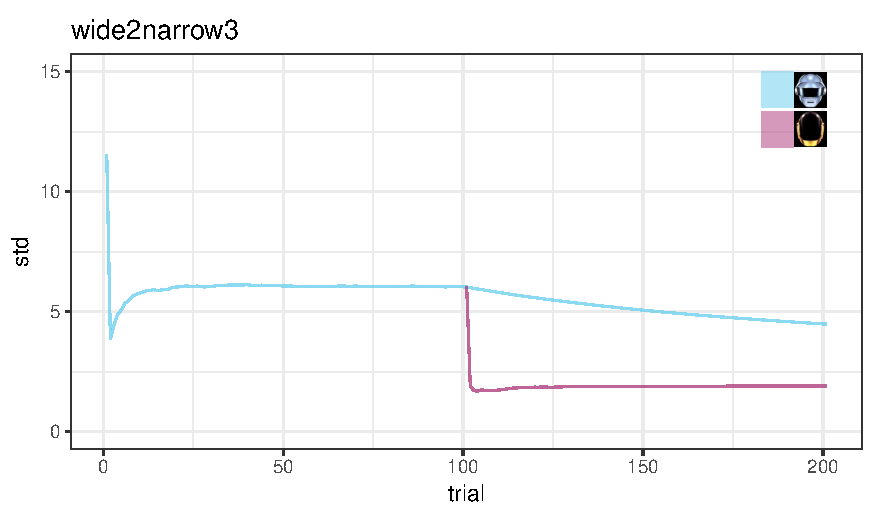
\includegraphics[width=\linewidth]{{comparisons1/avg_compare_robots_wide2narrow3-stub_0.1}.pdf}
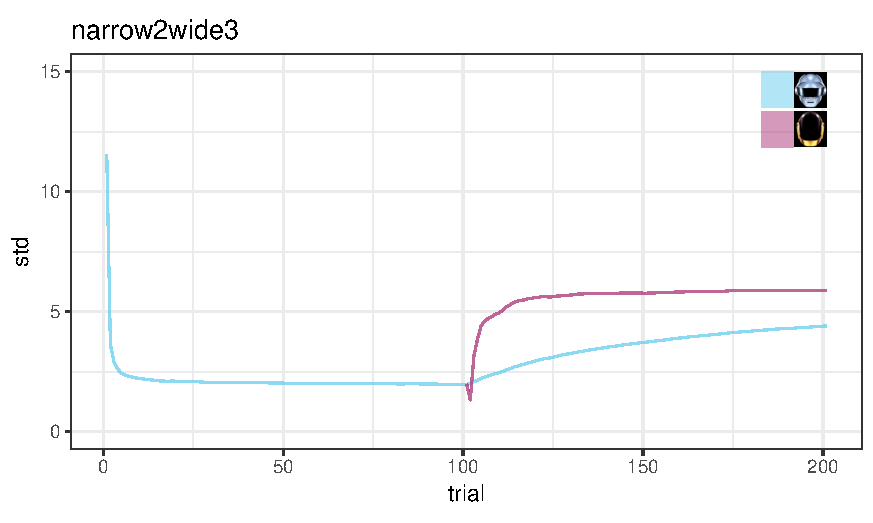
\includegraphics[width=\linewidth]{{comparisons1/avg_compare_robots_narrow2wide3-stub_0.1}.pdf}
\caption{Adaptation speed of the standard deviation for a robot after a
  change in the generation of the outcomes, compared with that of a robot
  that starts learning after the change, averaged over 100 experiments. The
  normals have same mean $17$ and standard deviations $6$ and
  $1.9$.}\label{fig:avg_comparison_robots_stds}
\end{figure}% done with exploration1.R
Figure~\ref{fig:avg_comparison_robots_stds} shows that this phenomenon is
even more striking if we average the sequences of standard deviations over
100 repetitions of such experiments.\mynote{L: so good?! must recheck the
  script.}

\begin{figure}[b!]
\centering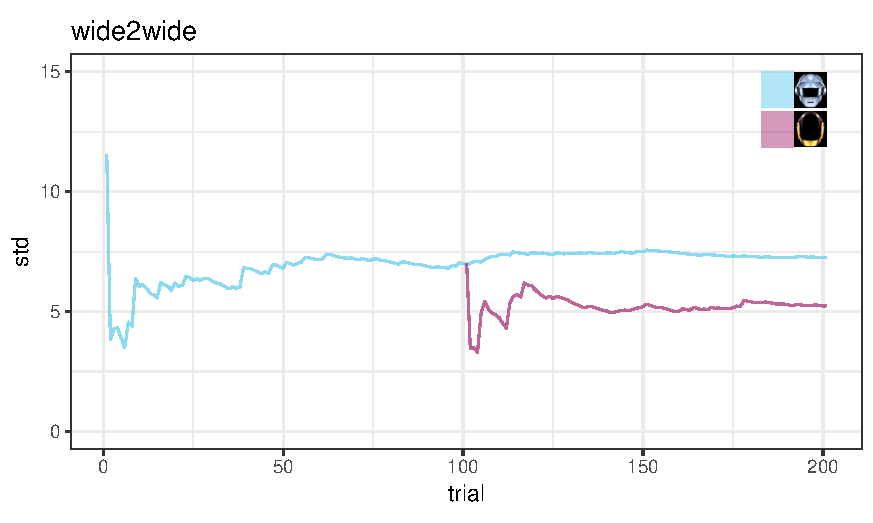
\includegraphics[width=\linewidth]{{comparisons1/compare_robots_wide2wide-stub_0.1}.pdf}
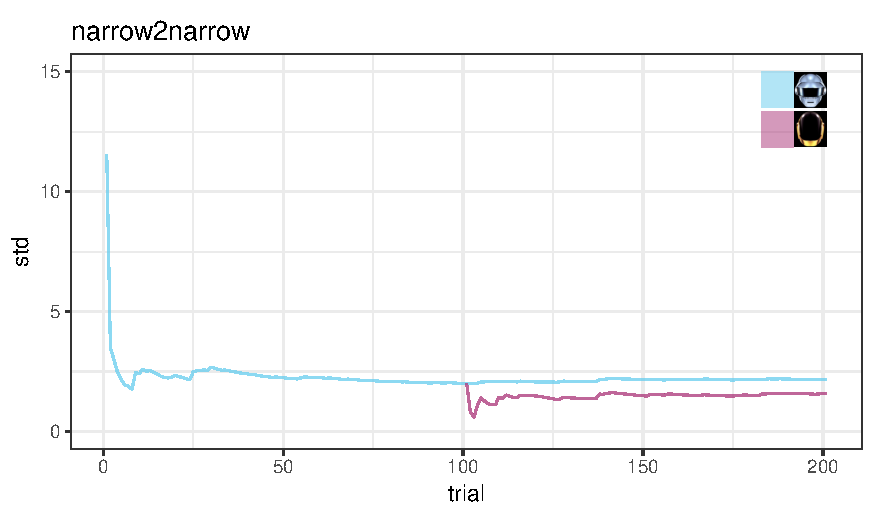
\includegraphics[width=\linewidth]{{comparisons1/compare_robots_narrow2narrow-stub_0.1}.pdf}
\caption{Adaptation speed of a robot after a change in the generation of
  the outcomes, compared with that of a robot that starts learning after
  the change.}\label{fig:comparison_robots_stds_2}
\end{figure}% done with exploration1.R

\clearpage

\section{Second study: exchangeable model with change-points}
\label{sec:second_study}

\subsection{The robot looks for change-points}
\label{sec:changepoints}

The robot of the previous study remembers past observations but not their
order. Said otherwise, it assumes that past frequencies are all that
matters for its inference. We now consider a new robot that takes the order
of observations into account in a simple way.

This new robot assumes that the sequence of observations is divided into
subsequences of contiguous observations. \emph{Within each subsequence} the
order of the observations doesn't matter: frequencies are sufficient
statistics, and the robot therefore uses an infinitely exchangeable model
with a Johnson-Dirichlet parameter density, as in the previous study. Only
observations within the subsequence contribute to the update of the
parameter density. Observations from other subsequences are irrelevant to
inferences within each subsequence, provided that the start point of that
subsequence is known. The stubbornness and frequency parameters are
therefore \enquote{reset} at the start of each subsequence.

The observations at which the subsequences start, called changepoints, are
guessed from the whole sequence of observations. The robot is effectively
considering all possible numbers and positions of changepoints. For
example, every observation could be a subsequence by itself, or all
observations could belong to just one subsequence -- which was the
assumption of the robot of the previous study. According to Bayes's
theorem, the robot assigns a probability to each possible division
proportionally to a prior times the product of the probabilities for the
data in each subsequence determined by that division, calculated with the
Johnson-Dirichlet model described above:
\begin{multline}
  \label{eq:explanation_P_group}
  \p(\ptext{particular division into subsequences} \| \ptext{data}, \yI)
  \propto{}\\
  \text{\footnotesize\emph{Johnson-Dirichlet}}\left\{\;
    \!\begin{aligned}
        &\quad\p(\ptext{data in 1st subsequence} \| \ptext{particular division}, \yI)
          \\
        &{}\times\p(\ptext{data in 2nd subsequence} \| \ptext{particular division}, \yI)
          \\
              &{}\times\dotsm
  \end{aligned}\right.\\
 {}\times \p(\ptext{particular division} \| \yI),
\end{multline}
where $\yI$ stands for other background assumptions. The final inference is
a combination of the inferences conditional on each possible division:
\begin{multline}
  \label{eq:explanation_group_mixed}
  \p(\ptext{new observation} \| \ptext{data}, \yI) \propto{}\\[\jot]
  \sum_{\mathclap{\text{all divisions}}}
  \p(\ptext{new observation} \| \ptext{division}, \ptext{data}, \yI)
\times  \p(\ptext{division} \| \ptext{data}, \yI),
\end{multline}
where the probability for the new observation given the division is
determined by the Johnson-Dirichlet model.

Adams \amp\ MacKay \citey{adamsetal2007} give an algorithm to do the
calculations above on-line as new observations are made. Before each
observation the algorithm saves the probability distribution for the
divisions~\eqref{eq:explanation_P_group}, which is used to calculate the
updated distribution with the new observation adjoined to the data.

For each observation $i$, consider the proposition \enquote{only the
  previous $r$ observations are relevant for the $i$th one}, denoted by
$R^{i}_{r}$. This proposition is equivalent to say that observations
$\set{i-r, i-r+1, \dotsc, i}$ form a subsequence. Obviously
$0\le r \le i-1$, where $i-1$ is the total number of observations before
the $i$th one; if $r=0$ then the $i$th observation is a changepoint,
starting a new subsequence, and no past data are relevant for its
inference. In symbols
\begin{multline}
  \label{eq:irrelevant_data_conditional_R}
  \p(D^{m+1}_{d_{m+1}} \|
  R^{m+1}_{r},  D^{m}_{d_{m}}, \dotsc, D^{1}_{d_{1}}, \yI)
  ={}\\
  \shoveright{\begin{cases}
  \p(D^{m+1}_{d_{m+1}} \|
    R^{m+1}_{r},  D^{m}_{d_{m}}, \dotsc, D^{m+1-r}_{d_{m+1-r}}, \yI)
    &\text{if $1\le r\le m$},
      \\[2\jot]
  \p(D^{m+1}_{d_{m+1}} \|
    R^{m+1}_{r}, \yI)
    &\text{if $r=0$},
  \end{cases}}
  \\
  \text{with probabilities given by the Johnson-Dirichlet
model~\eqref{eq:prediction_exchangeability}, \eqref{eq:JD_prior},
\eqref{eq:predictive_JD}.}
\end{multline}

The probability for the $(m+1)$th observation given the data can be thus
decomposed 
\begin{multline}
  \label{eq:prob_new_cond_R}
  \p(D^{m+1}_{d_{m+1}} \|
  D^{m}_{d_{m}}, \dotsc, D^{1}_{d_{1}}, \yI)
  =
  \frac{\p(D^{m+1}_{d_{m+1}}, D^{m}_{d_{m}} \|
    D^{m-1}_{d_{m-1}},\dotsc, D^{1}_{d_{1}}, \yI)}{
    \p(D^{m}_{d_{m}} \| D^{m-1}_{d_{m-1}}, \dotsc, D^{1}_{d_{1}}, \yI)}
=  {}\\[2\jot]
  \frac{\sum\limits_{r=0}^m
  \p(D^{m+1}_{d_{m+1}} \|
  R^{m+1}_{r},  D^{m}_{d_{m}}, \dotsc, D^{m+1-r}_{d_{m+1-r}}, \yI)
  \times
  \p(R^{m+1}_{r}, D^{m}_{d_{m}} \| D^{m-1}_{d_{m-1}} \dotsc, D^{1}_{d_{1}}, \yI)}{
\p(D^{m}_{d_{m}} \| D^{m-1}_{d_{m-1}} \dotsc, D^{1}_{d_{1}}, \yI)
}.
\end{multline}
The reason for this taking $D^{m}_{d_{m}}$ out of the conditional will be
apparent in a moment. Note that the denominator is the probability of the
previous observation given the previous data: in a recursive computation
this would have been computed in the preceding step.

The products in the sum contain the term given
by~\eqref{eq:irrelevant_data_conditional_R} and the joint probability for
$R^{m+1}_{r}, D^{m}_{d_{m}}$  given the previous data. This joint probability
 can be decomposed introducing $R^{m}_{s}$ for the previous observation:
\begin{multline}
  \label{eq:prob_R_and_last_decompose}
  \p(R^{m+1}_{r}, D^{m}_{d_{m}} \| D^{m-1}_{d_{m-1}}, \dotsc, D^{1}_{d_{1}}, \yI) 
 ={} \\[2\jot]
  \frac{\sum_{s=0}^{m-1}
    \p(R^{m+1}_{r}, D^{m}_{d_{m}}, R^{m}_{s}, D^{m-1}_{d_{m-1}}
    \| D^{m-2}_{d_{m-2}}, \dotsc, D^{1}_{d_{1}}, \yI)}{
\p(D^{m-1}_{d_{m-1}} \| D^{m-2}_{d_{m-2}}, \dotsc, D^{1}_{d_{1}}, \yI)}
  ={}\\[2\jot]
  % \begin{multlined}[b][0.9\textwidth]
  \begin{aligned}
    \frac{1}{\p(D^{m-1}_{d_{m-1}} \| D^{m-2}_{d_{m-2}}, \dotsc, D^{1}_{d_{1}}, \yI)}
  \sum_{s=0}^{m-1} \p(R^{m+1}_{r} \| R^{m}_{s}, \yI)
  \times{}\qquad\qquad&\\[\jot]
  \p(D^{m}_{d_{m}} \|
    R^{m}_{s}, D^{m-1}_{d_{m-1}} \dotsc, D^{m-s}_{d_{m-s}}, \yI)
    \times{}\qquad&\\[\jot]
 \p(R^{m}_{s}, D^{m-1}_{d_{m-1}} \|
  D^{m-2}_{d_{m-2}},\dotsc, D^{1}_{d_{1}}, \yI).&
  \end{aligned}
\end{multline}
The last expression contains four kinds of term. Let's analyse them.

1. The denominator is the probability for the $(m-1)$th observation given the
previous data. In a recursive algorithm this has been calculated in a
previous step.

2. The first factor within the sum was simplified using this assumption:
\begin{equation}
  \label{eq:prob_R_and_last_decompose}
  \p(R^{m+1}_{r} \|
  R^{m}_{s},  D^{m}_{d_{m}} \dotsc, D^{1}_{d_{1}}, \yI)
  = \p(R^{m+1}_{r} \|  R^{m}_{s},  \yI),
\end{equation}
which in words states that past data are irrelevant for guessing whether
the next observation starts a new subsequence or not, given that we know
how many data belong to the current subsequence, and given that we
\emph{don't} yet know the value of the next observation.

According to this assumption, past observations help us guessing whether
the next observation starts a new subsequence only if we can compare them
with it. If we don't know it, past data can't help us. This assumption
discards the possibility that particular values of past observations may
trigger the start of a new sequence. The length of the current subsequence,
$R^{m}_{s}$, is relevant in any case, because the next observation can only
start a new subsequence or continue the previous one, so that either $r=0$
or $r=s+1$:
\begin{equation}
  \label{eq:R_cond_R_simple}
  \p(R^{m+1}_{r} \| R^{m}_{s}, \yI) =
  \yrs(s)\,\delt_{r,0} + [1-\yrs(s)]\,\delt_{r,s+1} =
  \begin{cases}
    \yrs(s) & \text{for $r=0$},
    \\
    1-\yrs(s) &\text{for $r=s+1$},
    \\
    0 & \text{otherwise},
  \end{cases}
\end{equation}
which simplifies our calculations: in the
sum~\eqref{eq:prob_R_and_last_decompose} when $r\ge 1$ only the term
$s=r-1$ survives. In our study we assume that $\yrs(s)$ either is
independent of $s$ or increases with $s$, expressing our expectation that
subsequences shouldn't be too long. This last option is reasonable if the
participants were warned about the possibility of changepoints before the
experiment.

3. The second factor within the sum is given by the Johnson-Dirichlet
model, according to discussion of
\eqn~\eqref{eq:irrelevant_data_conditional_R}.

4. The last factor within the sum is analogous to the joint probability for
$R^{m+1}_{r}, D^{m}_{d_{m}}$, but calculated for the previous observation.
In a recursive scheme it would have been computed in the preceding step.


\bigskip

In a recursive scheme we also need some initial values.

For $m=0$ we have that $\p(D^{1}_{d_1} \| \yI)$ is given by the
Johnson-Dirichlet model, and $\p(R^{1}_{0} \| \yI)=1$ because the first
observation is trivially a changepoint. Owing to the certainty of $R^1_0$,
for $m=1$ we have
\begin{equation}
  \label{eq:initial_R2}
  \p(R^{2}_{r}, D^{1}_{d_{1}} \|  \yI)
  = \p(R^{2}_{r},R^{1}_{0}, D^{1}_{d_{1}} \|  \yI)
  = \p(R^{2}_{r} \| R^{1}_{0},  \yI) \times
  \p( D^{1}_{d_{1}} \|  \yI).
\end{equation}
With the probabilities above, from $m=2$ onward the recursion can be
calculated with
\eqns~\eqref{eq:irrelevant_data_conditional_R}--\eqref{eq:R_cond_R_simple}.


\subsection{The recursive algorithm}
\label{sec:adamsetal_algorithm}

The recursive algorithm to calculate
$\p(D^{m+1}_{d_{m+1}} \| D^{m}_{d_{m}}, \dotsc, D^{1}_{d_{1}}, \yI)$ is
shown in table~\ref{tab:adamsetal_algorithm}. For $m=0$ some initialization
steps are necessary.
\begin{table}[!b]
  \centering
  \caption{Initial steps of predictive algorithm}
  \label{tab:adamsetal_initial}
  \begin{tabularx}{\textwidth}{X}\hline
    \begin{enumerate}[label=0.\arabic*.,start=0]
    \item Set $\yN=0.01$, $\ynn_d=1/N$, $d\in\set{1,\dotsc,N}$
    \item For $d_1 \in \set{1,\dotsc,N}$ calculate
      \[A_1(d_1)\ defd
        \p(D^{1}_{d_{1}} \|  \yI) =\ynn_{d_1} \]
    \item Observe $d_1$
    \item Set $m=1$. For $r \in\set{0,1}$ calculate
      \[
        B_2(r) \defd \p(R^{2}_{r}, D^{1}_{d_1} \| \yI)
        =
        \begin{cases}
          \yrs(0) &\text{for $r=0$},\\ 1-\yrs(0)&\text{for $r=1$}
        \end{cases}
      \]
    \item  For $d_2 \in \set{1,\dotsc,N}$ calculate
      \[A_2(d_2) \defd
        \p(D^{2}_{d_{12}} \| D^{1}_{d_{1}}, \yI) =
        \ynn_{d_1} \]


    \item Keep $B_1(0)\equiv 1$ for next steps
    \item Observe $d_1$, set $m=1$
    \end{enumerate}
  \end{tabularx}
\end{table}

\begin{table}[!b]
  \centering
  \caption{Predictive algorithm}
  \label{tab:adamsetal_algorithm}
  \begin{tabularx}{\textwidth}{X}\hline
    \begin{enumerate}
      % \item Retrieve from memory
      %   \[ B_m(s) \defd \p(R^{m}_{s} \| D^{m-1}_{d_{m-1}} \dotsc,
      %     D^{1}_{d_{1}}, \yI),\qquad 0\le s \le m-1 \]
    \item\label{item:first_step}For $r \in \set{0,\dotsc, m}$:
      \begin{enumerate}[label*=\arabic*.]
      \item Calculate
        \[ \begin{multlined}[t][0.85\textwidth] C_{m+1}(r) \defd
            \p(R^{m+1}_{r} , D^{m}_{d_{m}} \| D^{m-1}_{d_{m-1}}, \dotsc,
            D^{1}_{d_{1}}, \yI) ={}\\[\jot]
       \shoveleft{\frac{1}{A_{m-1}(d_{m-1})} \times{}}\\\begin{cases}
          \sum_{s=0}^{m-1} \yrs(s) \times B_m(s,d_m) \times C_m(s) & \text{if $r=0$},
          \\[\jot]
          [1-\yrs(r-1)]  \times B_m(r-1,d_m) \times C_m(r-1)& \text{if $r\ge 1$}    
        \end{cases}
      \end{multlined}
    \]
      \item For $d_{m+1} \in \set{1,\dotsc,N}$, calculate
        \[ \begin{multlined}[][0.85\textwidth]
B_{m+1}(r,d_{m+1}) \defd \p(D^{m+1}_{d_{m+1}} \| R^{m+1}_{r}, D^{m}_{d_{m}},
          \dotsc, D^{m+1-r}_{d_{m+1-r}}, \yI) ={}\\[\jot]
         \frac{\yN\ynn_{d_{m+1}}+r\yff_{d_{m+1}}}{\yN + r},
       \end{multlined} \]
     where $\yff_{d_{m+1}}$ is the relative frequency of outcome $d_{m+1}$ in the previous $r$ observations
      % \item using the Johnson-Dirichlet model calculate (or retrieve from memory)
      %   \[ A_m(s) \defd \p(D^{m}_{d_{m}} \| R^{m}_{s}, D^{m-1}_{d_{m-1}}
      %     \dotsc, D^{m-s}_{d_{m-s}}, \yI)
      %   \]
  \end{enumerate}
\item For $d_{m+1} \in \set{1,\dotsc,N}$, calculate
  \[ \begin{multlined}[][0.85\textwidth]
      A_{m+1}(d_{m+1}) \defd \p(D^{m+1}_{d_{m+1}} \| D^{m}_{d_{m}}, \dotsc, D^{1}_{d_{1}}, \yI) ={}\\
    \frac{\sum_{r=0}^{m} B_{m+1}(r,d_{m+1}) \times
      C_{m+1}(r)}{A_{m}(d_{m})}
  \end{multlined}
\]
\item Observe $d_{m+1}$, 
\item Keep $A_{m+1}(d_{m+1})$ for the next two steps, and
  $B_{m+1}(r,d_{m+1})$, $C_{m+1}(r)$, $r\in\set{0,\dotsc,m}$ for the next step
\item Increase $m$ by $1$, go to step~\ref{item:first_step}
  \end{enumerate}
  \\\hline
\end{tabularx}
\end{table}

\clearpage

\section{Notes on hierarchic models}
\label{sec:notes_hierarchic}

\subsection{How hierarchic models get updated}
\label{sec:hierarchic_models}

The probability calculus allows for inferences that learn from data in
various degrees. We call \enquote{model} a particular way of doing
inference; each model is characterized by a particular capability of
learning from data. These capabilities arise from a hierarchy of groups
within groups of models.

At the bottom we have models that do not learn at all; we call them
\emph{independent}, because they assign independent probabilities to
different data. For example, denoting a particular independent model by
$\yth$ -- which could be the value of a parameter identifying the model --
and by $\yI$ all other knowledge or assumptions besides this model, we have
\begin{equation}
  \label{eq:indep_model}
  \pf(d_1,d_2 \| \yth, \yI) = \pf(d_1 \|\yth,\yI) \, \pf(d_2 \|\yth,\yI)
\end{equation}
for any two data $d_1$, $d_2$. This model does not learn because
\begin{equation}
  \label{eq:indep_model_nolearn}
  \pf(d_2\| d_1, \yth, \yI) = \pf(d_2 \|\yth,\yI),
\end{equation}
that is, under this model one set of data is always irrelevant for the
prediction of another set. The probability of an independent model given
data $d$ is
\begin{equation}
  \label{eq:prob_indep_model}
  \pf(\yth \| d, \yI)
  = \frac{
    \pf(d \|\yth,\yI) \, \pf(\yth \| \yI)
  }{
    \sum_{\yth}\pf(d \|\yth,\yI) \, \pf(\yth \| \yI)
  },
  % \equiv \frac{
  %   \pf(d \|\yth,\yI) \, \pf(\yth \| \yI)
  % }{
  %   \pf(d \|\yI)
  % },
\end{equation}
where $\pf(\yth \|\yI)$ is the probability over a range of such models
based only on knowledge $\yI$, and $\pf(d \|\yth,\yI)$ is the
\emph{likelihood} of the independent model given the data.

\medskip

We can introduce the capability of learning from data by considering a
collection $\set{\yth}$ of independent models, each having a probability,
and letting the data influence the probabilities of these models, rather
than the model themselves.

This particular model, based on a collection of independent models, is
usually called a \emph{parametric} model. Let us denote a particular
parametric model by $\ymu$. It is not independent because
\begin{equation}
  \label{eq:param_model}
  \begin{aligned}
  \pf(d_1,d_2 \| \ymu, \yI) &=
\sum_{\yth}
\pf(d_1,d_2 \|\yth,\ymu,\yI) \, \pf(\yth \| \ymu,\yI)
\\&\equiv
\sum_{\yth}
\pf(d_1 \|\yth,\ymu,\yI) \, \pf(d_2 \|\yth,\ymu,\yI)
 \, \pf(\yth \| \ymu,\yI),
  \end{aligned}
\end{equation}
which doesn't factorize unless $\pf(\yth \| \ymu,\yI)$ is a delta. The
first equality comes from the law of total probability. Such a model learns
because
\begin{subequations}
    \label{eq:param_model_learn}
  \begin{align}
    \pf(d_2 \| d_1, \ymu, \yI) &=
    \sum_{\yth}
    \pf(d_2 \|\yth,\ymu,\yI) \, \pf(\yth \| d_1, \ymu,\yI)
    \\
    \shortintertext{with}
    \pf(\yth \| d_1, \ymu,\yI)
    &= \frac{
      \pf(d_1 \|\yth,\ymu,\yI) \, \pf(\yth \| \ymu,\yI)
      }{
      \sum_{\yth} \pf(d_1 \|\yth,\ymu,\yI) \, \pf(\yth \| \ymu,\yI)
      },
  \end{align}
\end{subequations}
where we see that data $d_1$ affect not the probability of $d_2$ directly,
but the probability distribution for the various independent models. The
probability of a parametric model given data $d$ is
\begin{subequations}
  \label{eq:prob_indep_model}
  \begin{align}
    \pf(\ymu \| d, \yI)
    &= \frac{
      \pf(d \|\yth,\yI) \, \pf(\ymu \| \yI)
      }{
      \sum_{\ymu}\pf(d \|\ymu,\yI) \, \pf(\ymu \| \yI)
      }
    \\
    \shortintertext{with}
    \label{eq:param_model_likelihood}
    \pf(d \|\ymu,\yI)
    & =  
      \sum_{\yth}
      \pf(d \|\yth,\ymu,\yI) \, \pf(\yth \| \ymu,\yI).
  \end{align}
\end{subequations}
where $\pf(\ymu \|\yI)$ is the probability over a range of parametric
models based only on knowledge $\yI$. The last
expression~\eqref{eq:param_model_likelihood} is the \emph{likelihood} of
the model given the data, and we see that it's given by a mixture of
independent models.

\medskip

Equations~\eqref{eq:prob_indep_model} and~\eqref{eq:param_model} show that
a parametric model is constructed as an uncertainty over independent
models, and \eqn~\eqref{eq:param_model_learn} shows that data affect this
latter uncertainty. It is as if we were considering different ways of doing
inference, and inferring which of such inferences is most probable. Each
bottom inference is incapable to learn from data, but our inferences about
these inferences can learn from data.


We can proceed analogously and consider a collection $\set{\ymu}$ of
parametric models, each having a probability, and letting the data
influence this probability as well. The model constructed this way is
usually called a one-level hierarchic model -- even though we've seen that
a parametric model can also be considered as hierarchic. Let us denote such
a model by $\yh$. The probability of the data is
\begin{equation}
  \label{eq:hier_model}
  \begin{aligned}
  \pf(d_1,d_2 \| \yh, \yI) &=
\sum_{\ymu}
\pf(d_1,d_2 \|\ymu,\yh,\yI) \, \pf(\ymu \| \yh,\yI)
\\&\equiv
    \!\!\begin{multlined}[t][0.5\linewidth]
\sum_\ymu\biggl\{ \sum_{\yth}
\Bigl[ \prod_i\pf(d_i \|\yth,\ymu,\yh,\yI)\Bigr]\,
     \pf(\yth \| \ymu,\yh, \yI)\biggr\}\times{}\\
     \pf(\ymu \| \yh,\yI).
   \end{multlined}
  \end{aligned}
\end{equation}
Learning takes place this way:
\begin{subequations}
    \label{eq:hier_model_learn}
  \begin{align}
    \pf(d_2 \| d_1, \yh, \yI)
    &= \sum_{\ymu} \Bigl[\sum_{\yth}
      \pf(d_2 \|\yth,\ymu,\yh,\yI) \, \pf(\yth \| d_1, \ymu,\yh,\yI)
      \Bigr]\,
      \pf(\ymu \| d_1, \yh,\yI)
    \\
    \intertext{with}
      \begin{split}%[t][0.5\linewidth]
    \pf(\yth \| d_1, \ymu,\yh,\yI)
    &=\frac{
      \pf(d_1 \|\yth,\ymu,\yh,\yI) \, \pf(\yth \| \ymu,\yh,\yI)
      }{
      \sum_{\yth} \pf(d_1 \|\yth,\ymu,\yh,\yI) \, \pf(\yth \| \ymu,\yh,\yI)
    }
        \\[2\jot]
    &=\frac{
      \pf(d_1 \|\yth,\ymu,\yh,\yI) \, \pf(\yth \| \ymu,\yh,\yI)
      }{\pf(d_1 \| \ymu,\yh,\yI) },
    \end{split}\label{eq:update_h1}
      \\[3\jot]
    \pf(\ymu \| d_1, \yh,\yI)
    &= \frac{
      \pf(d_1 \|\ymu,\yh,\yI) \, \pf(\ymu \| \yh,\yI)
      }{
      \sum_{\ymu} \pf(d_1 \|\ymu,\yh,\yI) \, \pf(\ymu \| \yh,\yI)
      }.\label{eq:update_h2}
  \end{align}
\end{subequations}
Note that the denominator of the update formula~\eqref{eq:update_h1} for
$\yth$ is the updated probability~\eqref{eq:update_h2} for $\ymu$. Note
also that the space of independent models $\set{\yth}$ can be different for
different $\ymu$.

With a hierarchic model, it is as if we were considering different
\enquote{super-inferences} about ways of doing inferences, and inferring
which of such super-inferences is the most probable. This model learns from
the data in two ways: the data first give more probability to one or
another parametric model, and then give more probability to one or another
independent model within that parametric model. From another point of view
we can say that the data perform first a coarsen selection, and then a
finer one within each coarser selection.

We can of course multiply this kind of hierarchy ad libitum, proceeding as
we've done so far.

\subsection{Flattening hierarchic models}
\label{sec:flatten}

The subdivision of learning into two or more levels of different coarseness
can be very convenient, but mathematically it's always equivalent to one single
subdivision at the finest level. In other words, any hierarchic model can
always be rewritten as a parametric one. Let's see how, in the case of a
hierarchic model like~\eqref{eq:hier_model}.

We said that each parametric model $\ymu$ has a set
$\set{\yth} = \set{\yth}_{\ymu}$ of underlying independent models. For
example, in the case of real-valued data, one set could contain normal
distributions with the same variance and different means; another set could
contain uniform distributions with different supports; yet another set
could contain Cauchy distributions with the same location parameter and
different scale parameters. These sets can be pairwise disjoint,
overlapping, or even identical for different $\ymu$.

First of all let's consider each such set $\set{\yth}_{\ymu}$ as formally
distinct from all others for different $\ymu$. We consider the union of all
these sets, denoting a member of this union by $\yTh$:
\begin{equation}
  \label{eq:union_indip_models}
  \set{\yTh} \defd \bigcup_{\ymu}\set{\yth}_{\ymu}.
\end{equation}
Now consider the predictive probability~\eqref{eq:hier_model} for the
hierarchic model:
\begin{equation}
  \label{eq:hier_model_simple}
  \pf(d \| \yh, \yI) =
\sum_\ymu\biggl[ \sum_{\yth}
\pf(d \|\yth,\ymu,\yh,\yI)\,
     \pf(\yth \| \ymu,\yh, \yI)\biggr]\,
     \pf(\ymu \| \yh,\yI).
\end{equation}
If we decree that $\pf(\yTh \| \ymu,\yh,\yI) = 0$ if $\yTh \notin
\set{\yth}_{\ymu}$, we can extend the sum over $\yth$ (for fixed $\ymu$)
over all $\yTh$. Moreover, since $\yTh$ contains information about $\ymu$,
the latter becomes irrelevant in the conditional of the probability $\pf(d
\|\yth,\ymu,\yh,\yI)$. The predictive probability above then becomes
\begin{equation}
  \label{eq:hier_model_Theta}
  \begin{split}
  \pf(d \| \yh, \yI) &=
\sum_{\yTh}
\pf(d \|\yTh,\yh,\yI)\, \sum_\ymu 
     \pf(\yTh \| \ymu,\yh, \yI)\,
     \pf(\ymu \| \yh,\yI),
\\ &= \sum_{\yTh}
\pf(d \|\yTh,\yh,\yI)\,
     \pf(\yTh \| \yh, \yI),
   \end{split}
\end{equation}
where the last equality follows from the law of total probability. What's
important in the last formula is that the probability
$\pf(d \|\yTh,\yh,\yI)$ factorizes over conjunctions of data; that is, it
is an independent model. The model above is therefore just a parametric
model.

The last step consists in joining together into a single value all those
values of $\yTh$ which lead to identical predictive distributions
$\pf(d \|\yTh,\yh,\yI)$. The probability $\pf(\yTh \| \yh, \yI)$  for such
a value will be the sum of the probability for the various equivalent values.

\mynote{to be cont'd}



%\setlength{\intextsep}{0.5ex}% with wrapfigure
%\begin{figure}[p!]%{r}{0.4\linewidth} % with wrapfigure
%  \centering\includegraphics[trim={12ex 0 18ex 0},clip,width=\linewidth]{maxent_saddle.png}\\
%\caption{***}\label{fig:comparison_a5}
%\end{figure}% exp_family_maxent.nb


\iffalse
\begin{acknowledgements}
  \ldots to Mari \amp\ Miri for continuous encouragement and affection, and
  to Buster Keaton and Saitama for filling life with awe and inspiration.
  To the developers and maintainers of \LaTeX, Emacs, AUC\TeX, Open Science
  Framework, Python, Inkscape, Sci-Hub for making a free and unfiltered
  scientific exchange possible.
%\rotatebox{15}{P}\rotatebox{5}{I}\rotatebox{-10}{P}\rotatebox{10}{\reflectbox{P}}\rotatebox{-5}{O}.
%\sourceatright{\autanet}
\end{acknowledgements}
\fi

%\appendixpage
%\appendix

%%%%%%%%%%%%%%% BIB %%%%%%%%%%%%%%%

\defbibnote{prenote}{{\footnotesize (\enquote{de $X$} is listed under D,
    \enquote{van $X$} under V, and so on, regardless of national
    conventions.)\par}}
% \defbibnote{postnote}{\par\medskip\noindent{\footnotesize% Note:
%     \arxivp \mparcp \philscip \biorxivp}}

\printbibliography[prenote=prenote%,postnote=postnote
]


\end{document}
---------- cut text ----------------


% This distribution for $R^{m+1}_r$ represents the robot's guess of whether
% the new observation starts a new subsequence or whether it is part of the
% previous subsequence, and of how long that subsequence is. It can be
% calculated recursively by introducing $R^{m}_{s}$ for the previous
% observation:
% \begin{equation}
%   \label{eq:prob_R_and_last_decompose2}
%     \p(R^{m+1}_{r}\| D^{m}_{d_{m}}, \dotsc, D^{1}_{d_{1}}, \yI) 
%   % &=\sum_{s=0}^{m-1}
%   % \p(R^{m+1}_{r},R^{m}_{s},\|
%   % D^{m}_{d_{m}}, \dotsc, D^{1}_{d_{1}}, \yI)
%   % \\
% =\sum_{s=0}^{m-1}\p(R^{m+1}_{r} \| R^{m}_{s}, \yI)
%   \times
%   \p(R^{m}_{s} \|
%   D^{m-1}_{d_{m-1}} \dotsc, D^{1}_{d_{1}}, \yI).
% % &\!\begin{multlined}[b][0.7\textwidth]
% %   =\sum_{s=0}^{m-1}\p(R^{m+1}_{r} \| R^{m}_{s}, \yI)
% %   \times{}\\
% %   \p(D^{m}_{d_{m}} \| R^{m}_{s},
% %   D^{m-1}_{d_{m-1}} \dotsc, D^{m-s}_{d_{m-s}}, \yI)
% %   \times{}\\
% %   \p(R^{m}_{s} \|
% %   D^{m-1}_{d_{m-1}} \dotsc, D^{1}_{d_{1}}, \yI).
% %           \end{multlined}
% %   \end{aligned}
% \end{equation}
% Let's examine the two factors in the sum.

%%% Local Variables: 
%%% mode: LaTeX
%%% TeX-PDF-mode: t
%%% TeX-master: t
%%% End: 
